\documentclass[ROB,english]{tumbeamer}

% If you load additional packages, do so in packages.sty as figures are build
% as standalone documents and you may want to have effect on them, too.

% Folder structure:
% .
% ├── beamermods.sty                  % depricated an will be removed soon
% ├── compile                         % remotely compile slides
% ├── figures                         % all figures go here
% │   └── schichtenmodelle_osi.tikz   % each .tikz or .tex is a target
% ├── include                         % create your document here
% │   ├── example.tex                 % example document
% │   └── slides.tex                  % make document wide changes here
% ├── lit.bib                         % literature
% ├── Makefile
% ├── moeptikz.sty                    % fancy networking symbols
% ├── packages.sty                    % load additional packages there
% ├── pics                            % binary pcitures go here
% ├── slides.tex                      % main document (may be more than one)
% ├── tumbeamer.cls
% ├── tumcolor.sty                    % TUM color definitions
% ├── tumcontact.sty                  % TUM headers and footers
% ├── tumlang.sty                     % TUM names and language settings
% └── tumlogo.sty                     % TUM logos

% Configure author, title, etc. here:
\documentclass[ROB,english]{tumbeamer}

% If you load additional packages, do so in packages.sty as figures are build
% as standalone documents and you may want to have effect on them, too.

% Folder structure:
% .
% ├── beamermods.sty                  % depricated an will be removed soon
% ├── compile                         % remotely compile slides
% ├── figures                         % all figures go here
% │   └── schichtenmodelle_osi.tikz   % each .tikz or .tex is a target
% ├── include                         % create your document here
% │   ├── example.tex                 % example document
% │   └── slides.tex                  % make document wide changes here
% ├── lit.bib                         % literature
% ├── Makefile
% ├── moeptikz.sty                    % fancy networking symbols
% ├── packages.sty                    % load additional packages there
% ├── pics                            % binary pcitures go here
% ├── slides.tex                      % main document (may be more than one)
% ├── tumbeamer.cls
% ├── tumcolor.sty                    % TUM color definitions
% ├── tumcontact.sty                  % TUM headers and footers
% ├── tumlang.sty                     % TUM names and language settings
% └── tumlogo.sty                     % TUM logos

% Configure author, title, etc. here:
\documentclass[ROB,english]{tumbeamer}

% If you load additional packages, do so in packages.sty as figures are build
% as standalone documents and you may want to have effect on them, too.

% Folder structure:
% .
% ├── beamermods.sty                  % depricated an will be removed soon
% ├── compile                         % remotely compile slides
% ├── figures                         % all figures go here
% │   └── schichtenmodelle_osi.tikz   % each .tikz or .tex is a target
% ├── include                         % create your document here
% │   ├── example.tex                 % example document
% │   └── slides.tex                  % make document wide changes here
% ├── lit.bib                         % literature
% ├── Makefile
% ├── moeptikz.sty                    % fancy networking symbols
% ├── packages.sty                    % load additional packages there
% ├── pics                            % binary pcitures go here
% ├── slides.tex                      % main document (may be more than one)
% ├── tumbeamer.cls
% ├── tumcolor.sty                    % TUM color definitions
% ├── tumcontact.sty                  % TUM headers and footers
% ├── tumlang.sty                     % TUM names and language settings
% └── tumlogo.sty                     % TUM logos

% Configure author, title, etc. here:
\documentclass[ROB,english]{tumbeamer}

% If you load additional packages, do so in packages.sty as figures are build
% as standalone documents and you may want to have effect on them, too.

% Folder structure:
% .
% ├── beamermods.sty                  % depricated an will be removed soon
% ├── compile                         % remotely compile slides
% ├── figures                         % all figures go here
% │   └── schichtenmodelle_osi.tikz   % each .tikz or .tex is a target
% ├── include                         % create your document here
% │   ├── example.tex                 % example document
% │   └── slides.tex                  % make document wide changes here
% ├── lit.bib                         % literature
% ├── Makefile
% ├── moeptikz.sty                    % fancy networking symbols
% ├── packages.sty                    % load additional packages there
% ├── pics                            % binary pcitures go here
% ├── slides.tex                      % main document (may be more than one)
% ├── tumbeamer.cls
% ├── tumcolor.sty                    % TUM color definitions
% ├── tumcontact.sty                  % TUM headers and footers
% ├── tumlang.sty                     % TUM names and language settings
% └── tumlogo.sty                     % TUM logos

% Configure author, title, etc. here:
\input{include/slides}

\begin{document}

% For lecture mode, you may want to build one set of slides per chapter but
% with common page numbering. If so,
% 1) create a new .tex file for each chapter, e.g. slides_chapN.tex,
% 2) set the part counter to N-1 (assuming chapters start at 0), and
% 3) and name your chapter by using the \part{} command.
%\setcounter{part}{-1}
%\part{Organisatorisches und Einleitung}

% Include source files from ./include (or ./include/chapN).
\input{include/rstdp}

% Include markdown source from ./pandoc
%\input{pandoc/example}

% Comment out if you do not want a bibliography
\begin{frame}[allowframebreaks]
    \bibliographystyle{abbrv}
    \setbeamertemplate{bibliography item}[text]
    \footnotesize
    \bibliography{lit}
\end{frame}

\end{document}



\begin{document}

% For lecture mode, you may want to build one set of slides per chapter but
% with common page numbering. If so,
% 1) create a new .tex file for each chapter, e.g. slides_chapN.tex,
% 2) set the part counter to N-1 (assuming chapters start at 0), and
% 3) and name your chapter by using the \part{} command.
%\setcounter{part}{-1}
%\part{Organisatorisches und Einleitung}

% Include source files from ./include (or ./include/chapN).

\begin{frame}
	\frametitle{Task: Target Tracking}
	\begin{columns}
		\column{0.5\linewidth}
			\begin{itemize}
				\item <1-> Target Tracking SNN
				\item <2-> Prevent collisions with walls
				\item <2-> Obstacle Avoidance SNN
				\item <2-> R-STDP learning rule
			\end{itemize}
		\column{0.5\linewidth}
			\begin{overprint}
				\onslide<1>
				\begin{figure}
					\centering
					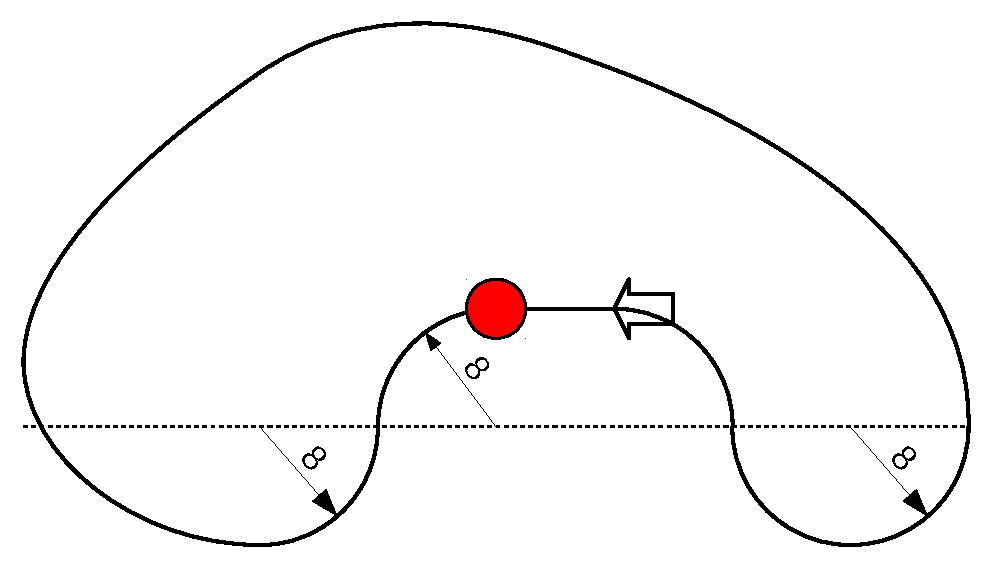
\includegraphics[width=\textwidth]{img/eval_path_tf.pdf}
					\caption{Target tracking SNN evaluation environment.}
					\label{fig:eval_path_tf}
				\end{figure}
				\onslide<2>
				\begin{figure}
					\centering
					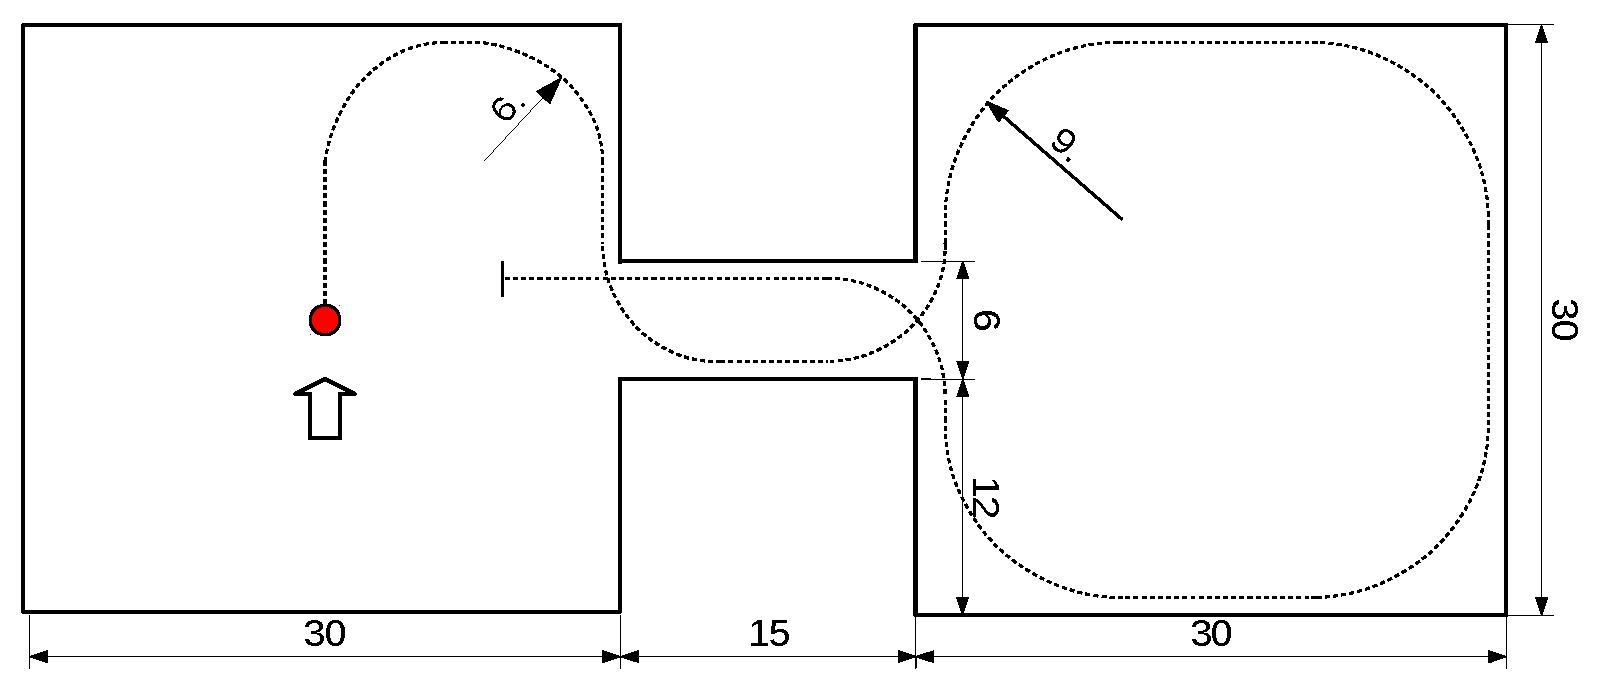
\includegraphics[width=\textwidth]{img/eval_path.pdf}
					\caption{Evaluation environment}
					\label{fig:eval_path}
				\end{figure}
			\end{overprint}
	\end{columns}
\end{frame}

\begin{frame}
	\frametitle{Target Following SNN}
	\begin{columns}
		\column{0.5\linewidth}
			\begin{itemize}
				\item <1-> Infrared image $32 \times 32 $ pixel resolution
				\item <2-> Image preprocessing
				\item <3-> 64 Poisson input neurons
				\item <3-> Feed forward architecture
				\item <3-> Left and Right LIF output neurons
			\end{itemize}
		\column{0.5\linewidth}
			\begin{overprint}
				\onslide<1>
				\begin{figure}
					\centering
					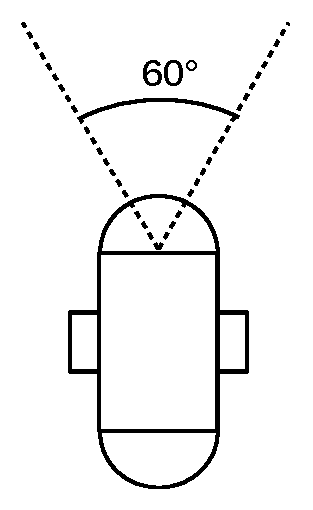
\includegraphics[height=0.7\textheight]{img/sensors_a.pdf}
					\caption{Infrared vision sensor}
					\label{fig:sensor_a}
				\end{figure}
				\onslide<2>
				\begin{figure}
					\centering
					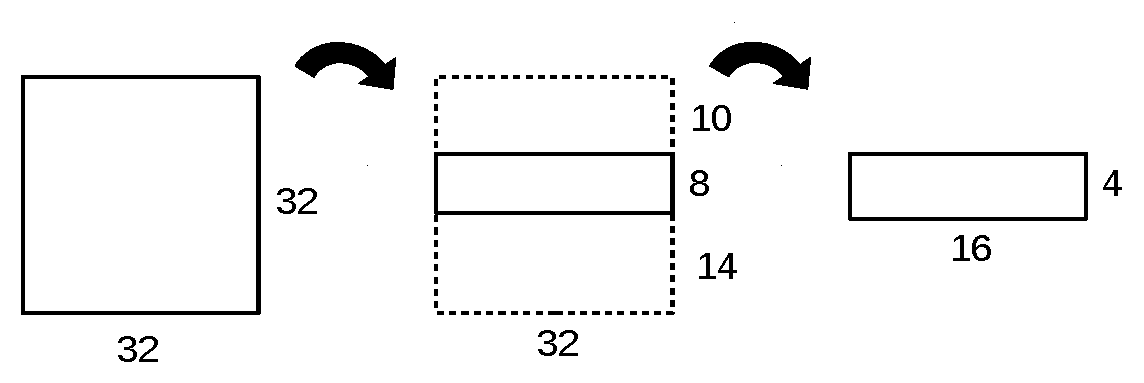
\includegraphics[width=\textwidth]{img/img_pre.pdf}
					\caption{Image preprocessing in 3 steps}
					\label{fig:img_pre}
				\end{figure}
				\onslide<3>
				\begin{figure}
					\centering
					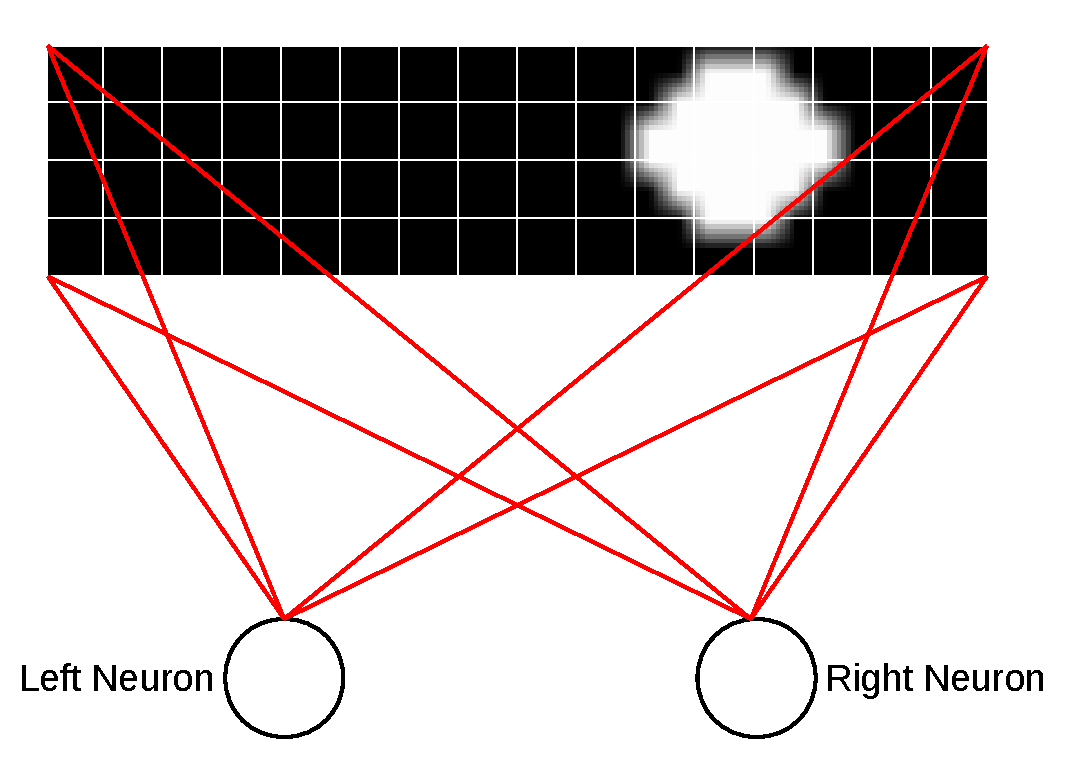
\includegraphics[width=\textwidth]{img/arch_tf.pdf}
					\caption{Target following SNN architecture}
					\label{fig:arch_tf}
				\end{figure}
			\end{overprint}
	\end{columns}
\end{frame}

\begin{frame}
	\frametitle{Target Following SNN cont.}
	\begin{columns}
		\column{0.5\linewidth}
			\begin{itemize}
				\item <1-> Output interpreted as angle
				\item <2-> Reward depends on Angle between head module and target
				\item <3-> Left and right neuron get the opposite rewards of each other
			\end{itemize}
		\column{0.5\linewidth}
			\begin{overprint}
				\onslide<1>
				\[decode\left(n_{spikes}\right) = \frac{n_{spikes}}{n_{max}}\]
				\[\alpha = \alpha_{max} \left(n_l - n_r\right)\]
				\[\alpha_t = c \alpha + \left(1 - c\right) \alpha_{t-1}\]
				\onslide<2>
				\begin{figure}
					\centering
					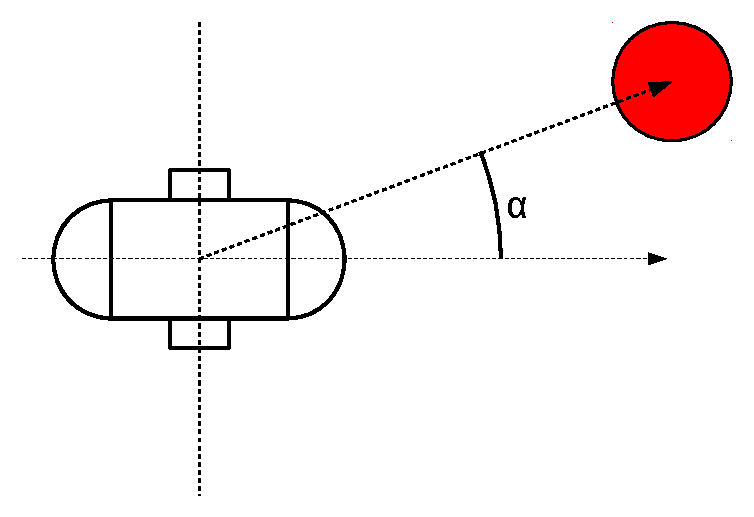
\includegraphics[width=\textwidth]{img/angle.pdf}
					\caption{Angle between robot head module and target.}
					\label{fig:angle}
				\end{figure}
				\onslide<3>
				\begin{figure}
					\centering
					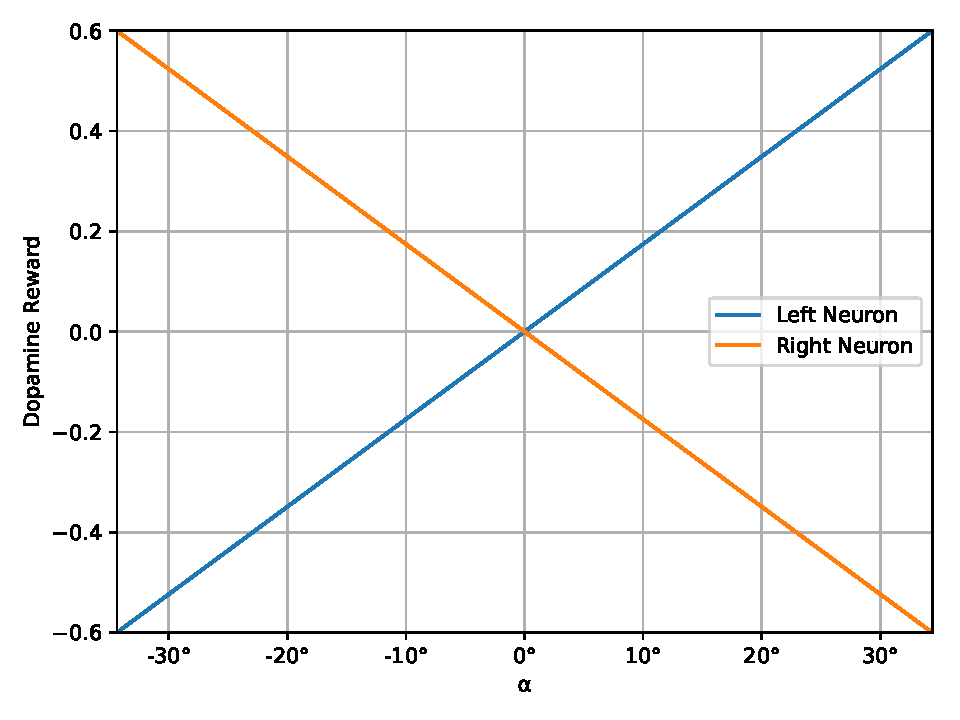
\includegraphics[width=\textwidth]{img/angle_reward.pdf}
					\caption{Target following reward function}
					\label{fig:angle_reward}
				\end{figure}
			\end{overprint}
	\end{columns}
\end{frame}

\begin{frame}
	\frametitle{Obstacle Avoidance SNN}
	\begin{columns}
		\column{0.5\linewidth}
			\begin{itemize}
				\item <1-> Four proximity sensors
				\item <2-> Proximity data preprocessing
				\item <3-> 4 Poisson input neurons
				\item <3-> Feed forward architecture
				\item <3-> Left and right LIF output neurons
			\end{itemize}
		\column{0.5\linewidth}
			\begin{overprint}
				\onslide<1>
				\begin{figure}
					\centering
					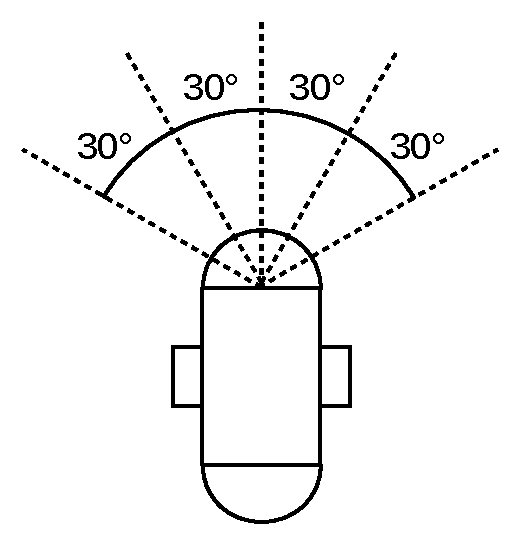
\includegraphics[height=0.7\textheight]{img/sensors_b.pdf}
					\caption{Proximity sensors}
					\label{fig:sensor_b}
				\end{figure}
				\onslide<2>
				\begin{itemize}
					\item Data in range $[0;3]$
					\item Mapped to range $[0:1]$
					\item $0$: No obstacle or at maximum distance
					\item $1$: Close obstacle
				\end{itemize}
				\onslide<3>
				\begin{figure}
					\centering
					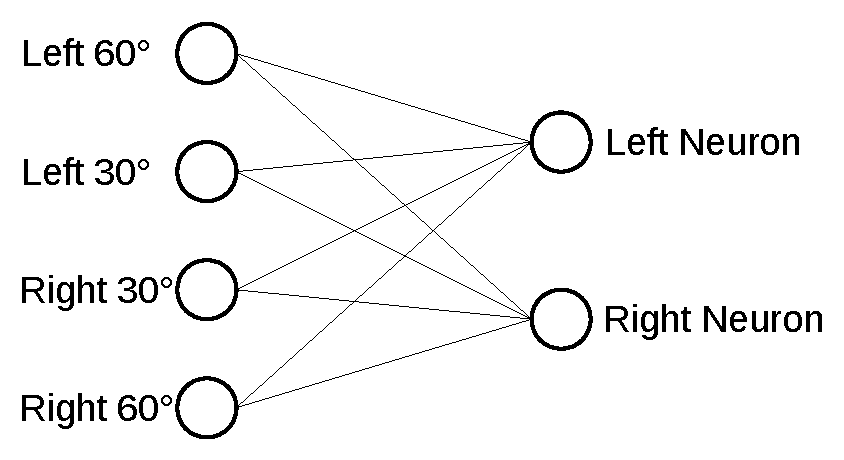
\includegraphics[width=\textwidth]{img/arch_oa.pdf}
					\caption{Obstacle avoidance SNN architecture}
					\label{fig:arch_oa}
				\end{figure}
			\end{overprint}
	\end{columns}
\end{frame}

\begin{frame}
	\frametitle{Obstacle Avoidance SNN cont.}
	\begin{columns}
		\column{\linewidth}
			\begin{itemize}
				\item <1-> Output interpreted as angle
				\[decode\left(n_{spikes}\right) = \frac{n_{spikes}}{n_{max}}\]
				\[\alpha = \alpha_{max} \left(n_l - n_r\right)\]
				\item <2-> Event based rewards on Episode failure
				\item <2-> Left and right neuron get the opposite rewards of each other
				\item <2-> 4 Reward cases, collision and target lost, obstacle left or right side
			\end{itemize}			
	\end{columns}
\end{frame}

\begin{frame}
	\frametitle{Controller Selection}
	\begin{itemize}
		\item Both SNN return an angle
		\item Select one as command for the robot
		\item Choose the target tracking angle except if that brings the robot too close to an obstacle.
	\end{itemize}
\end{frame}

\begin{frame}
	\frametitle{Training Environment}
	\begin{columns}
		\column{\linewidth}
			\begin{overprint}
				\onslide<1>
				\begin{figure}
					\centering
					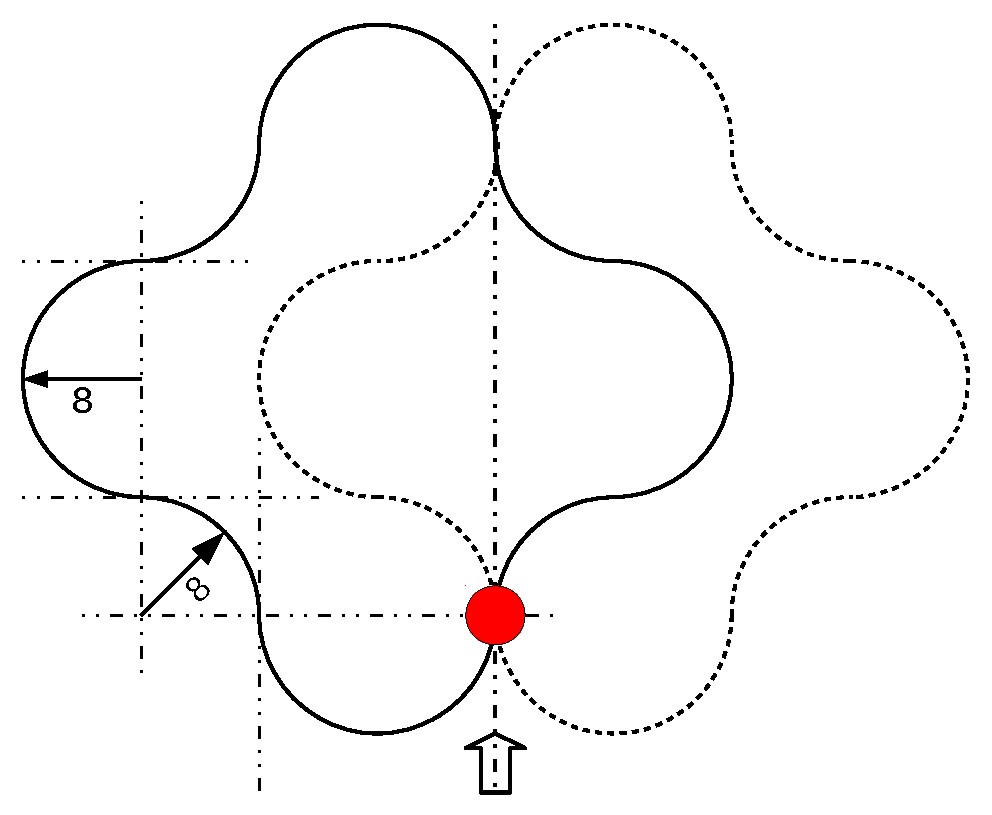
\includegraphics[height=0.6\textheight]{img/tf_training_path.pdf}
					\caption{Target tracking SNN training path}
					\label{fig:tf_training_path}
				\end{figure}
			\end{overprint}
	\end{columns}
\end{frame}

\begin{frame}
	\frametitle{Training Target Tracking SNN}
	\begin{figure}
		\centering
		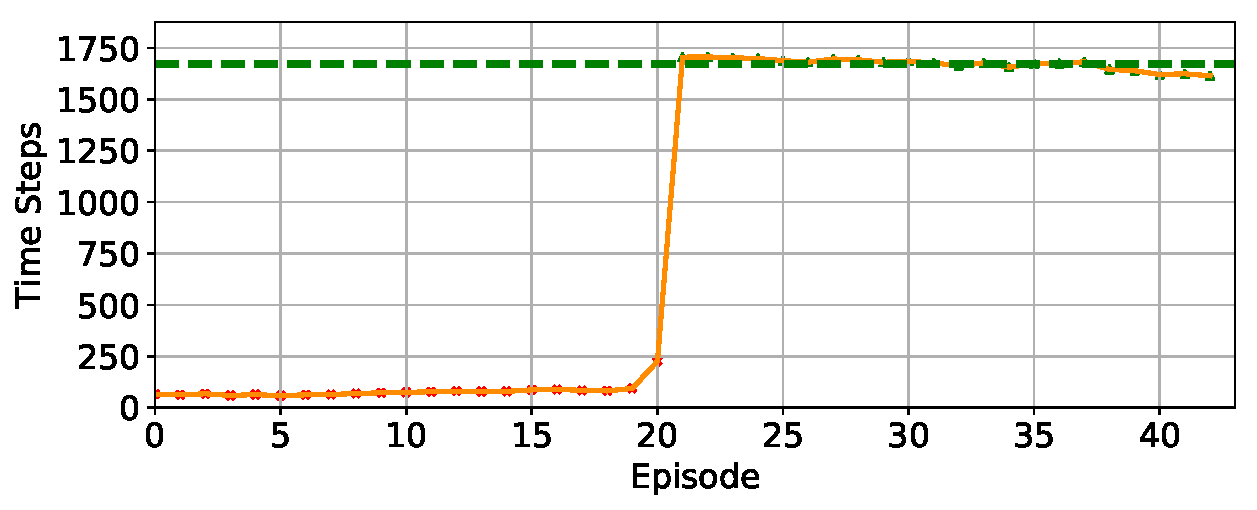
\includegraphics[width=\textwidth]{img/success_tf.pdf}
		\caption{Target Tracking Training}
		\label{fig:tf_success}
	\end{figure}
\end{frame}

\begin{frame}
	\frametitle{Training Target Tracking SNN}
	\begin{figure}
		\centering
		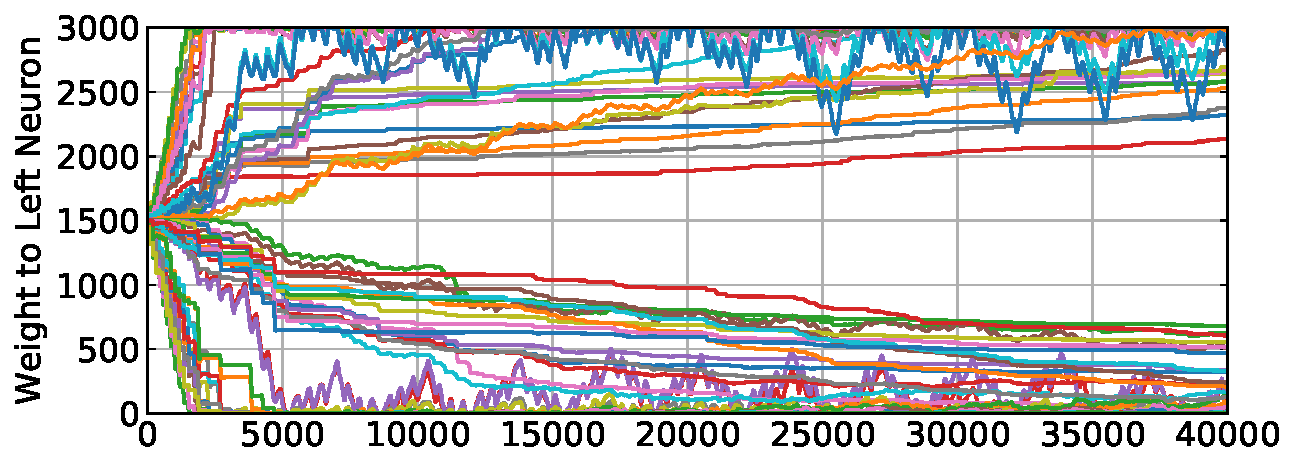
\includegraphics[width=\textwidth]{img/weight_change_left_tf.pdf}
		\caption{Left neuron weight changes during training}
		\label{fig:tf_weight_changes_left}
	\end{figure}
\end{frame}

\begin{frame}
	\frametitle{Training Environment}
	\begin{columns}
		\column{\linewidth}
			\begin{overprint}
				\begin{figure}
					\centering
					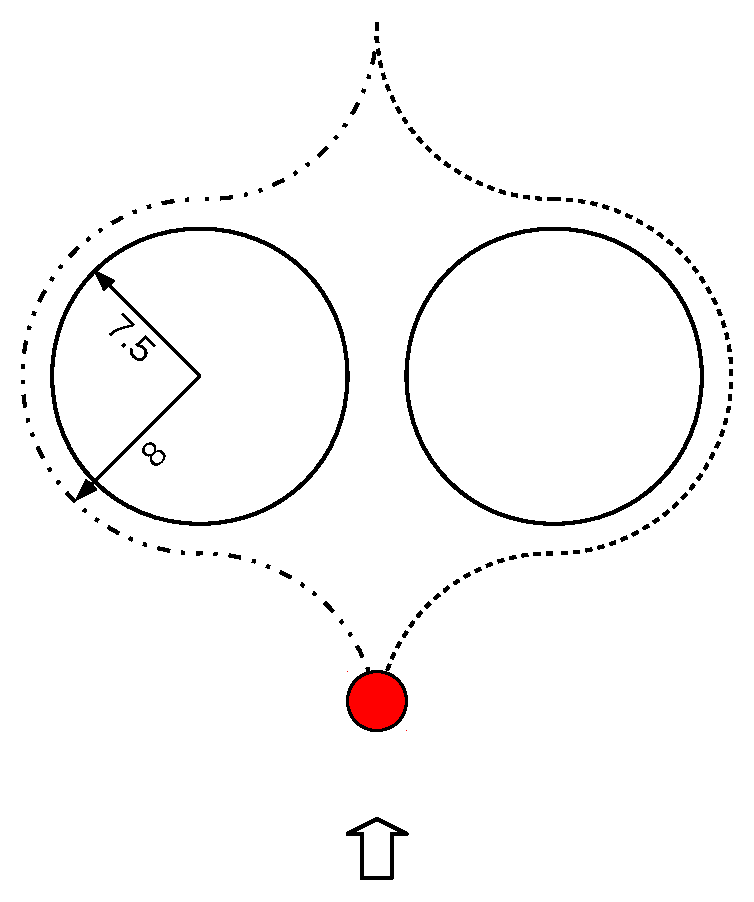
\includegraphics[height=0.6\textheight]{img/oa_training_path.pdf}
					\caption{Obstacle avoidance SNN training path}
					\label{fig:oa_training_path}
				\end{figure}
			\end{overprint}
	\end{columns}
\end{frame}

\begin{frame}
	\frametitle{Training Obstacle Avoidance SNN}
	\begin{figure}
		\centering
		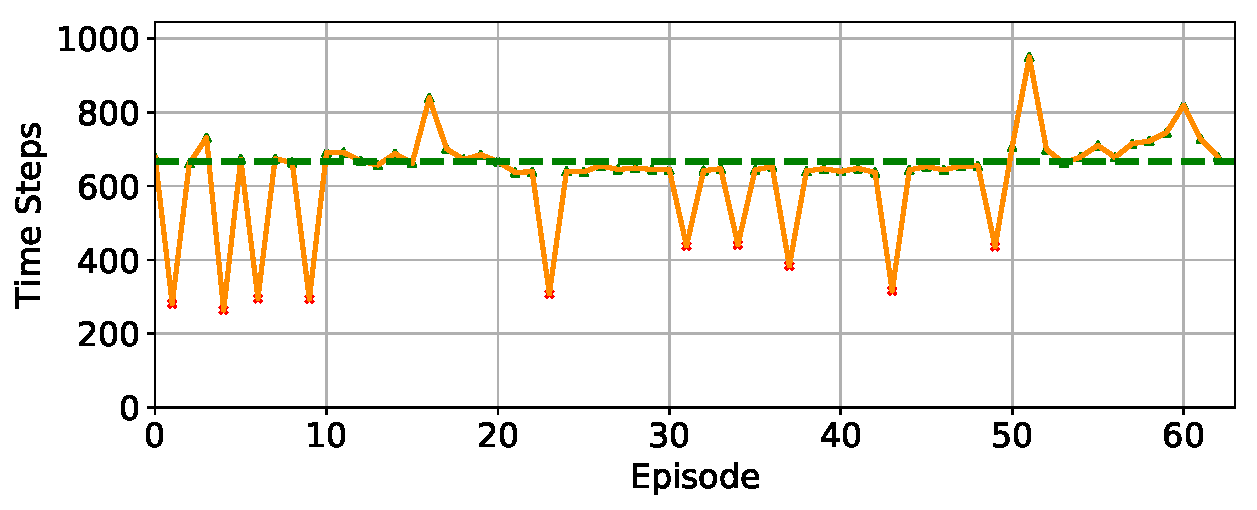
\includegraphics[width=\textwidth]{img/success_oa.pdf}
		\caption{Obstacle Avoidance Training}
		\label{fig:oa_success}
	\end{figure}
\end{frame}

\begin{frame}
	\frametitle{Training Target Tracking SNN}
	\begin{figure}
		\centering
		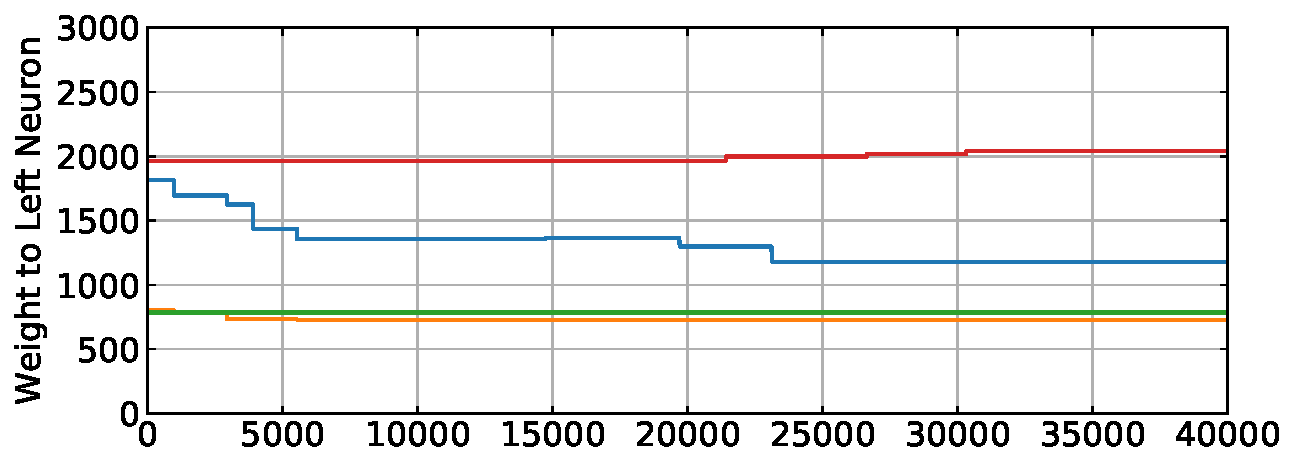
\includegraphics[width=\textwidth]{img/weight_change_left_oa.pdf}
		\caption{Left neuron weight changes during training}
		\label{fig:oa_weight_changes_left}
	\end{figure}
\end{frame}

\begin{frame}
	\frametitle{Evaluation}
	\begin{itemize}
		\item <1-> Average error $ e = \SI{7,39}{\degree}$
		\item <2-> Average error $ e = \SI{8.71}{\degree}$
	\end{itemize}
	\begin{overprint}
		\onslide<1>
		\begin{figure}
			\centering
			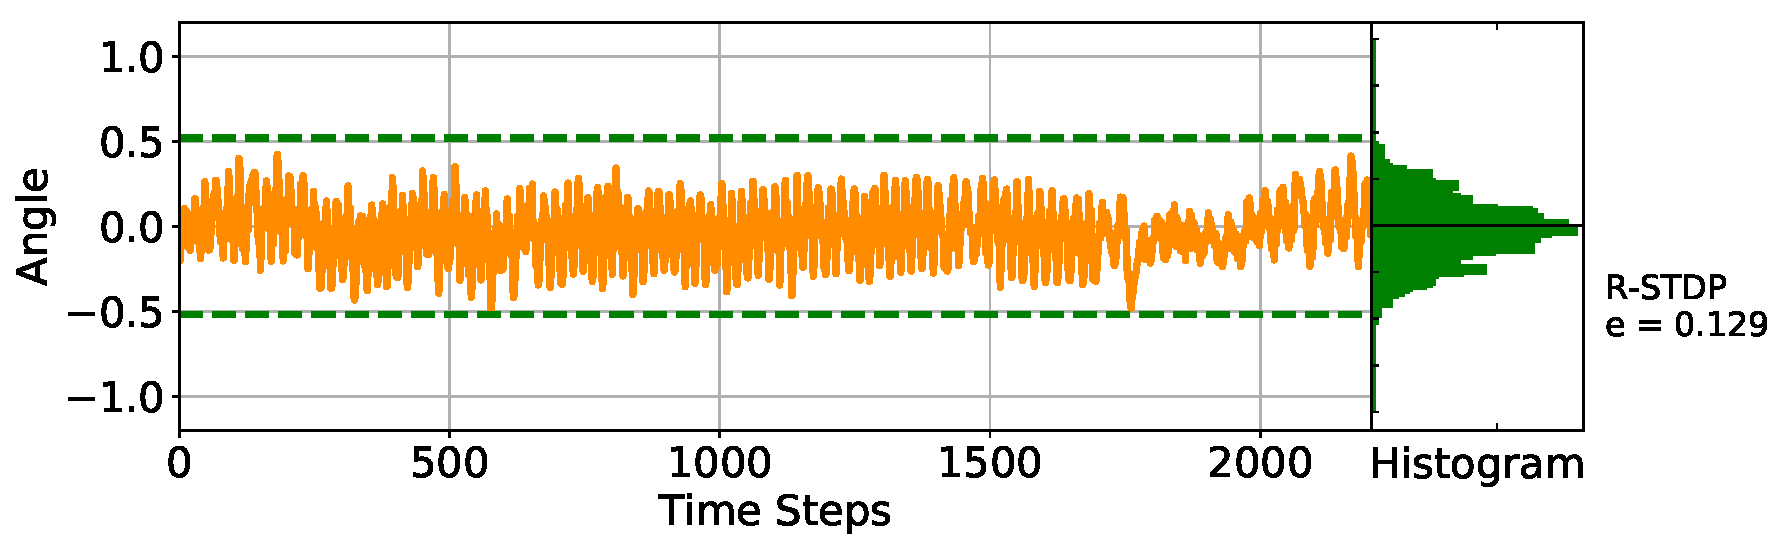
\includegraphics[width=\textwidth]{img/performance_tf.pdf}
			\caption{Performance on Target Following Task}
			\label{fig:Performance_tf}
		\end{figure}
		\onslide<2>
		\begin{figure}
			\centering
			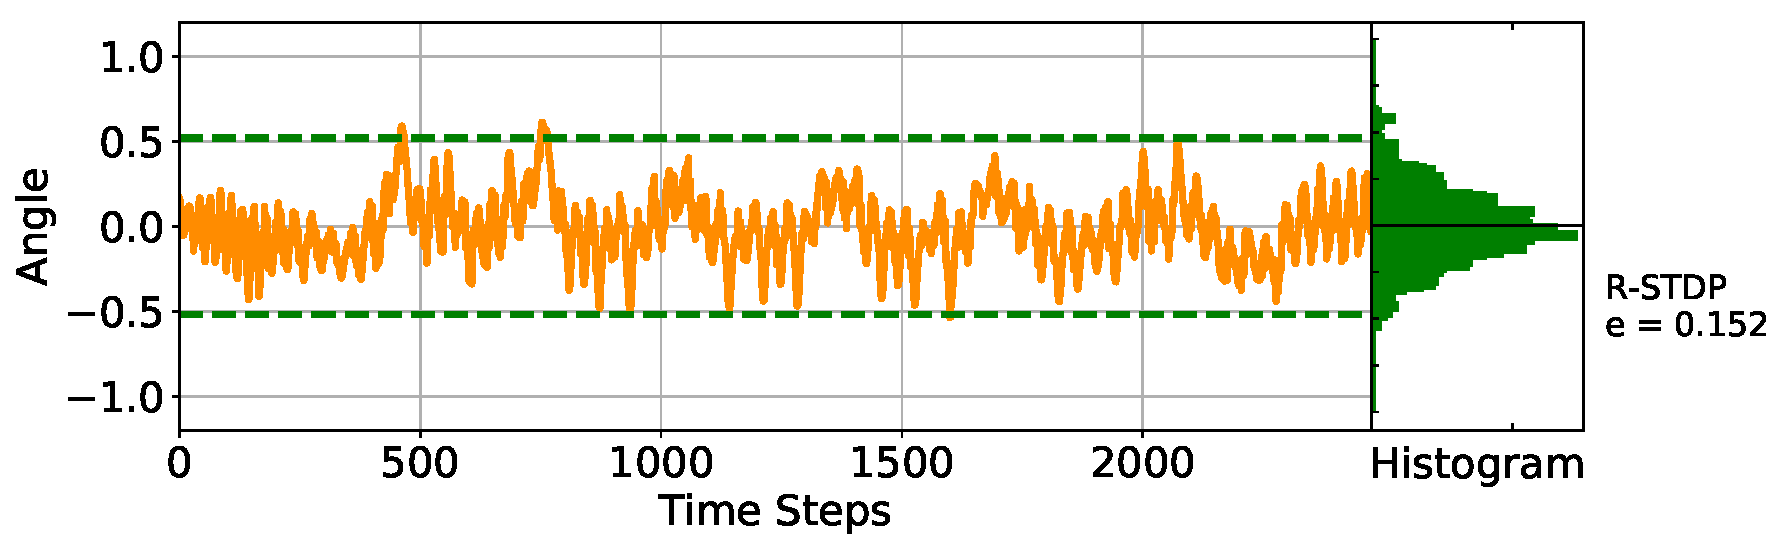
\includegraphics[width=\textwidth]{img/performance_oa.pdf}
			\caption{Performance on Target Tracking and Obstacle Avoidance Task}
			\label{fig:Performance_oa}
		\end{figure}
	\end{overprint}
\end{frame}

\begin{frame}
	\frametitle{title}
\end{frame}


% Include markdown source from ./pandoc
%
\begin{frame}
	\frametitle{Galileo - Weg zum Start}
	\begin{itemize}
		\item Antrag genehmigt am 14.4.1977
		\item Erforschung von Jupiter und seinen Monden
		\item Flugbahn\"anderungen durch Monde
		\item Raumsonde und Atmosph\"arenprobe
		\item Geplanter Start 1982
	\end{itemize}
\end{frame}


\begin{frame}
	\frametitle{Verteiltes Rechnen auf Galileo}
	\begin{itemize}
		\item CDS - Command and Data Subsystem
		\item DPU - Data Processing Units
		\item AACS - Attitude and Articulation Control Subsystem
		\item Atmosph\"arensonde System
		\item Systemsynchronisation über Clock alle 2.5 Millisekunden
	\end{itemize}
\end{frame}

\begin{frame}
	\frametitle{CDS - Command and Data Subsystem}
	\begin{itemize}
		\item CDS besteht aus HLM, zwei LLM und Bus
		\item HLM - High-level module
		\begin{itemize}
			\item RCA 1802, Speicher, Bussystem
			\item Bus kontrolle, System\"uberwachung
		\end{itemize}
		\item LLM - Low-level modules
		\begin{itemize}
			\item RCA 1802, Speicher
			\item \"Uberwachung der Raumsonde, Atmosph\"arenprobe
		\end{itemize}
		\item Identisches Backup
	\end{itemize}
\end{frame}

\begin{frame}
	\frametitle{CDS Software}
	\begin{itemize}
		\item Assembler mit Macros (IF, DO, ASSIGN)
		\item Vordergrund Prozesse z.B. Selbstest, Bus Kontrolle
		\item Hintergrundprozesse 6 Virtuelle Maschinen
		\item Jede VM hat einen Programmstack im Speicher
		\item VM mit höherer Priorität bekommen mehr Rechenzeit
	\end{itemize}
\end{frame}

\begin{frame}
	\frametitle{DPU - Data Processing Unit}
	\begin{itemize}
		\item Eine DPU pro Experiment
		\item RCA 1802 und Speicher
		\item Antenne im Time-Sharing Betrieb
		\item Anfallende Daten gehen im n\"achsten Zeitslot zur Erde
		\item Assembler
		\item Eine DPU wurde mit FORTH programmiert
	\end{itemize}
\end{frame}

\begin{frame}
	\frametitle{AACS - Attitude and Articulation Control Subsystem}
	\begin{itemize}
		\item Basiert auf Voyager's System
		\item Zwei redundande ATAC - Applied Technologies Advanced Computer
		\item Orientierung der Sonde im Raum
		\item Ausrichtung der Instrumentenplattform
		\item Z\"undung der Triebwerke
	\end{itemize}
\end{frame}

\begin{frame}
	\frametitle{AACS}
	\begin{itemize}
		\item 16 Bit Computer bestehend aus vier 4 Bit AMD 2900 bitslice Prozessoren
		\item 9,5 MHz
		\item HAL/S Programme
		\item Assembler Betriebssystem GRACOS - Galileo Real-time Attitude Control Operating System
		\item SEU Problem anf\"allig
		\item Ohne Versp\"atung beim Start Ausfall wegen Io m\"oglich
	\end{itemize}
\end{frame}

\begin{frame}
	\frametitle{RCA 1802}
	\begin{itemize}
		\item Strahlengeh\"artet Silizium auf Saphir
		\item 3.2 MHz Taktrate
		\item RISC mit 8 Bit Befehlen, nur 16 Befehle
		\item 16 Register zu je 16 Bit
		\item Programmcounter und Indexregister kann frei gew\"ahlt werden
		\item I/O direkt vom und in den Speicher
	\end{itemize}
\end{frame}


\begin{frame}
\frametitle{Start}
	\begin{itemize}
		\item Start verschoben in 1982, 1985 und 1986
		\begin{itemize}
			\item Verz\"ogerungen beim Spaceshuttle Programm
			\item Pr\"asident Reagan
			\item Challenger Katastrophe
		\end{itemize}
		\item Folgen jeder Verschiebung
		\begin{itemize}
			\item Neue Route zum Jupiter
			\item Umbau der Raumsonde
		\end{itemize}
		\item Start am 18.10.1989
	\end{itemize}
\end{frame}

\begin{frame}
\frametitle{Flug zum Jupiter \"Ubersicht}
	\begin{itemize}
		\item Dauer 6 Jahre
		\item Schwung holen an Venus und zwei mal an Erde
		\item Vorbeiflug an Planetoiden Gaspra und Ida
		\item Primärmission beginnt beim Jupiter
	\end{itemize}
\end{frame}


\begin{frame}
	\begin{figure}
		\centering
		\includegraphics[width=0.5\textwidth]{pics/venus.jpg}
		\caption{Vorbeiflug an Venus am 14.2.1990\cite{nasaphoto}}
		\label{VENUS}
	\end{figure}
\end{frame}

\begin{frame}
	\begin{figure}
		\centering
		\includegraphics[width=0.5\textwidth]{pics/erde0.jpg}
		\caption{Vorbeiflug an Erde am 12.12.1990\cite{nasaphoto}}
		\label{ERDE0}
	\end{figure}
\end{frame}

\begin{frame}
	\begin{figure}
		\centering
		\includegraphics[width=0.5\textwidth]{pics/gaspra.jpg}
		\caption{Vorbeiflug an Planetoiden Gaspra am 29.10.1991\cite{nasaphoto}}
		\label{GASPRA}
	\end{figure}
\end{frame}

\begin{frame}
	\begin{figure}
		\centering
		\includegraphics[width=0.7\textwidth]{pics/ida.jpg}
		\caption{Vorbeiflug an Planetoiden Ida und sein Mond Dactyl am 28.8.1991\cite{nasaphoto}}
		\label{IDA}
	\end{figure}
\end{frame}

\begin{frame}
	\begin{figure}
		\centering
		\includegraphics[width=0.7\textwidth]{pics/jupiter.jpg}
		\caption{Komet Shoemaker-Levy 9 schl\"agt auf Jupiter ein. 22.7.1994\cite{nasaphoto}}
		\label{JUPITER}
	\end{figure}
\end{frame}

\begin{frame}
	\begin{figure}
		\centering
		\includegraphics[width=0.8\textwidth]{pics/monde.jpg}
		\caption{Die Galileischen Monde Io, Europa, Ganymede, und Callisto\cite{nasaphoto}}
		\label{GALILEO_MONDE}
	\end{figure}
\end{frame}

\begin{frame}
	\frametitle{Probleme wärend der Reise zum Jupiter}
	\begin{itemize}
		\item HGA - Hochgewinnantenne Entfaltet sich nicht
		\item NGA - Niedriggewinnantenne nur \"Ubertragungsrate 10 Bit/s
		
		\item Bandrekorder reagiert für 18 Stunden nicht
		\item Leichter Schaden f\"uhrt zu 16\% weniger Speicher
	\end{itemize}
\end{frame}

\begin{frame}
	\frametitle{Probleml\"osung durch Software Updates}
	\begin{itemize}
		\item Antenne Paketbasierter Betrieb
		\item DPU's erstellen und w\"ahlen Pakete
		\item Bilder werden auf Bandrekorder zwischengespeichert
		\item CDS bearbeitet und komprimiert Bilder
		\item DCT - Diskrete Cosinustransformation zur verlustbehaftete Bildkomprimierung (JPEG)
	\end{itemize}
\end{frame}

\begin{frame}
\frametitle{Prim\"armission}
	\begin{itemize}
		\item 7.5.1995 bis 7.12.1997
		\item 11 Orbits um Jupiter
		\item Relativ naher Vorbeiflug an je einem Mond
		\item Unerwartet große Treibstoffreserven nach Mission
	\end{itemize}
\end{frame}

\begin{frame}
	\frametitle{Verl\"angerungen}
	\begin{itemize}
		\item GEM - Galileo Europa Mission
		\begin{itemize}
			\item 8.12.1997 bis 31.12.1999
			\item 14 Orbits, 7 Vorbeifl\"uge an Europa
		\end{itemize}
		\item GMM - Galileo Millennium Mission
		\begin{itemize}
			\item 1.2.2000 bis 21.9.2003
			\item Probleme h\"aufen sich
			\item Riskante Vorbeifl\"uge an Io
		\end{itemize}
	\end{itemize}
\end{frame}

\begin{frame}
	\frametitle{Vielen Dank f\"ur Ihre Aufmerksamkeit!}
	\begin{figure}
		\centering
		\includegraphics[width=0.6\textwidth]{pics/number_of_computers.png}
		\caption{xkcd Comic\cite{xkcd}}
		\label{NUMBER_OF_COMPUTERS}
	\end{figure}
\end{frame}


% Comment out if you do not want a bibliography
\begin{frame}[allowframebreaks]
    \bibliographystyle{abbrv}
    \setbeamertemplate{bibliography item}[text]
    \footnotesize
    \bibliography{lit}
\end{frame}

\end{document}



\begin{document}

% For lecture mode, you may want to build one set of slides per chapter but
% with common page numbering. If so,
% 1) create a new .tex file for each chapter, e.g. slides_chapN.tex,
% 2) set the part counter to N-1 (assuming chapters start at 0), and
% 3) and name your chapter by using the \part{} command.
%\setcounter{part}{-1}
%\part{Organisatorisches und Einleitung}

% Include source files from ./include (or ./include/chapN).

\begin{frame}
	\frametitle{Task: Target Tracking}
	\begin{columns}
		\column{0.5\linewidth}
			\begin{itemize}
				\item <1-> Target Tracking SNN
				\item <2-> Prevent collisions with walls
				\item <2-> Obstacle Avoidance SNN
				\item <2-> R-STDP learning rule
			\end{itemize}
		\column{0.5\linewidth}
			\begin{overprint}
				\onslide<1>
				\begin{figure}
					\centering
					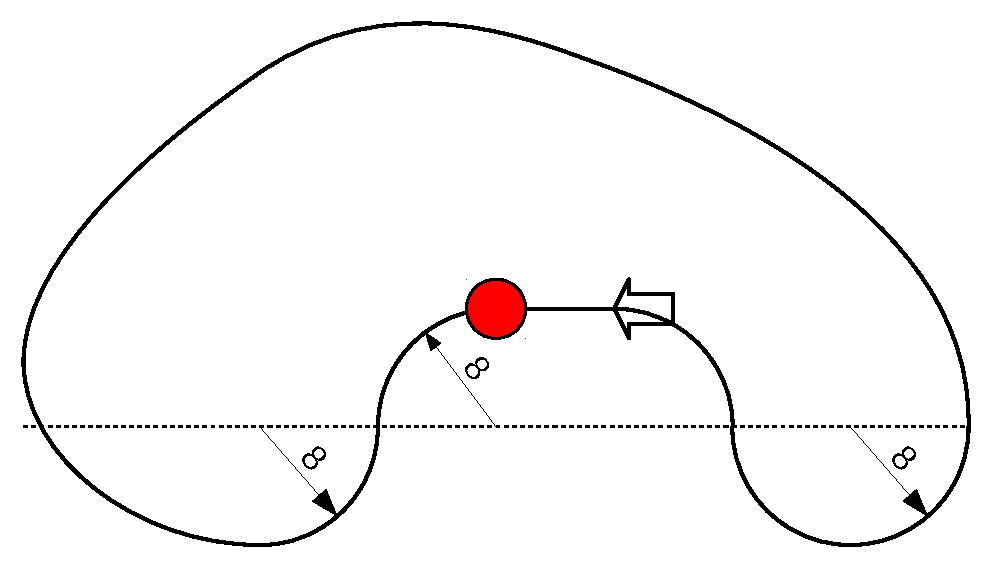
\includegraphics[width=\textwidth]{img/eval_path_tf.pdf}
					\caption{Target tracking SNN evaluation environment.}
					\label{fig:eval_path_tf}
				\end{figure}
				\onslide<2>
				\begin{figure}
					\centering
					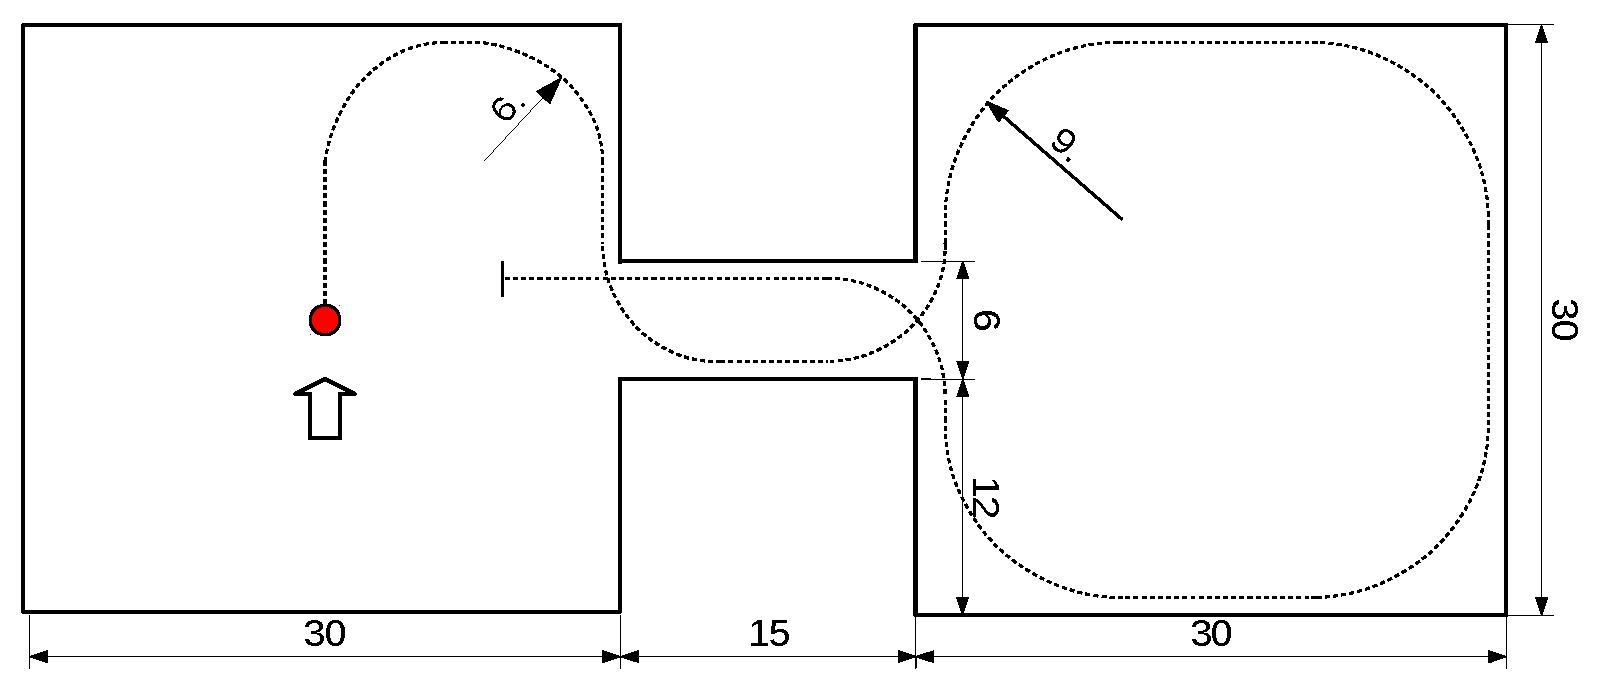
\includegraphics[width=\textwidth]{img/eval_path.pdf}
					\caption{Evaluation environment}
					\label{fig:eval_path}
				\end{figure}
			\end{overprint}
	\end{columns}
\end{frame}

\begin{frame}
	\frametitle{Target Following SNN}
	\begin{columns}
		\column{0.5\linewidth}
			\begin{itemize}
				\item <1-> Infrared image $32 \times 32 $ pixel resolution
				\item <2-> Image preprocessing
				\item <3-> 64 Poisson input neurons
				\item <3-> Feed forward architecture
				\item <3-> Left and Right LIF output neurons
			\end{itemize}
		\column{0.5\linewidth}
			\begin{overprint}
				\onslide<1>
				\begin{figure}
					\centering
					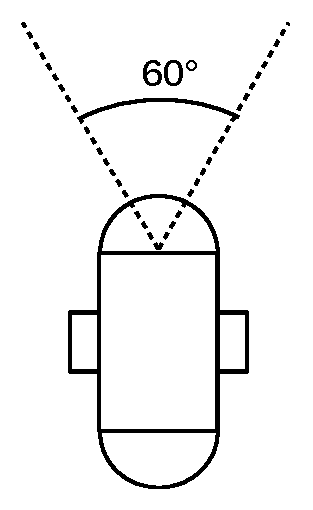
\includegraphics[height=0.7\textheight]{img/sensors_a.pdf}
					\caption{Infrared vision sensor}
					\label{fig:sensor_a}
				\end{figure}
				\onslide<2>
				\begin{figure}
					\centering
					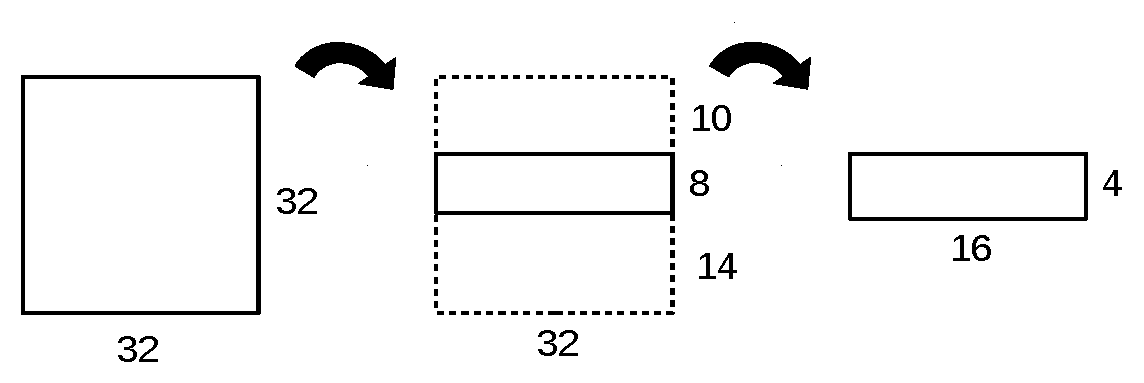
\includegraphics[width=\textwidth]{img/img_pre.pdf}
					\caption{Image preprocessing in 3 steps}
					\label{fig:img_pre}
				\end{figure}
				\onslide<3>
				\begin{figure}
					\centering
					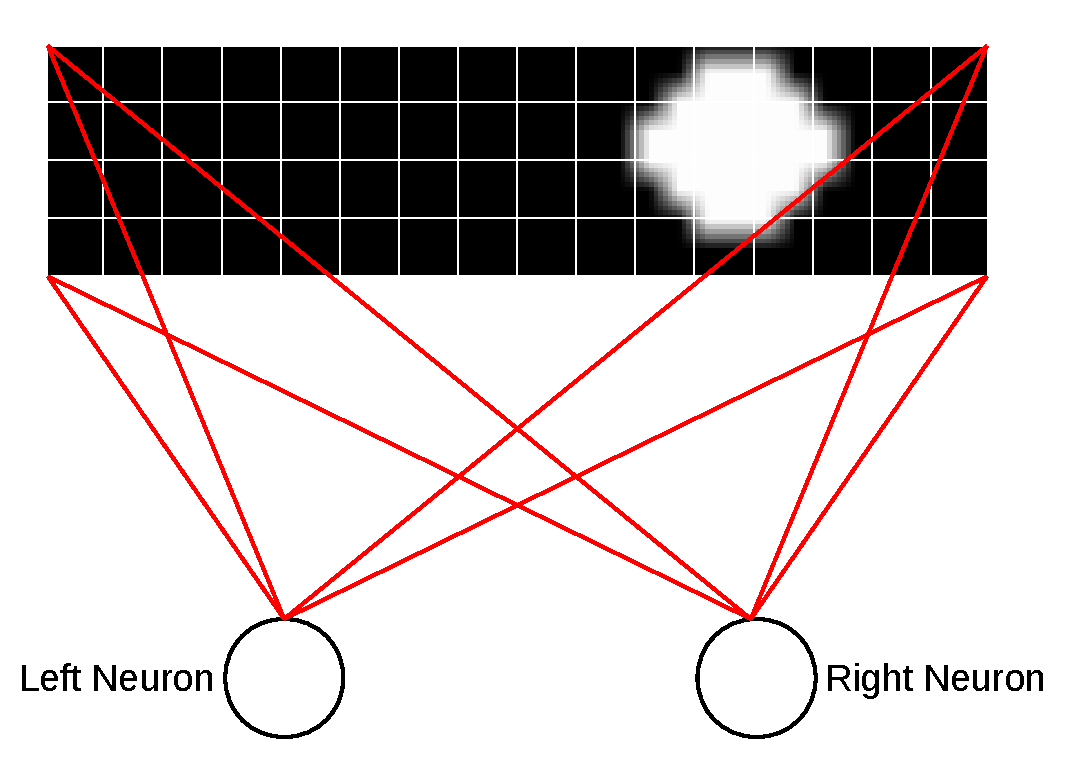
\includegraphics[width=\textwidth]{img/arch_tf.pdf}
					\caption{Target following SNN architecture}
					\label{fig:arch_tf}
				\end{figure}
			\end{overprint}
	\end{columns}
\end{frame}

\begin{frame}
	\frametitle{Target Following SNN cont.}
	\begin{columns}
		\column{0.5\linewidth}
			\begin{itemize}
				\item <1-> Output interpreted as angle
				\item <2-> Reward depends on Angle between head module and target
				\item <3-> Left and right neuron get the opposite rewards of each other
			\end{itemize}
		\column{0.5\linewidth}
			\begin{overprint}
				\onslide<1>
				\[decode\left(n_{spikes}\right) = \frac{n_{spikes}}{n_{max}}\]
				\[\alpha = \alpha_{max} \left(n_l - n_r\right)\]
				\[\alpha_t = c \alpha + \left(1 - c\right) \alpha_{t-1}\]
				\onslide<2>
				\begin{figure}
					\centering
					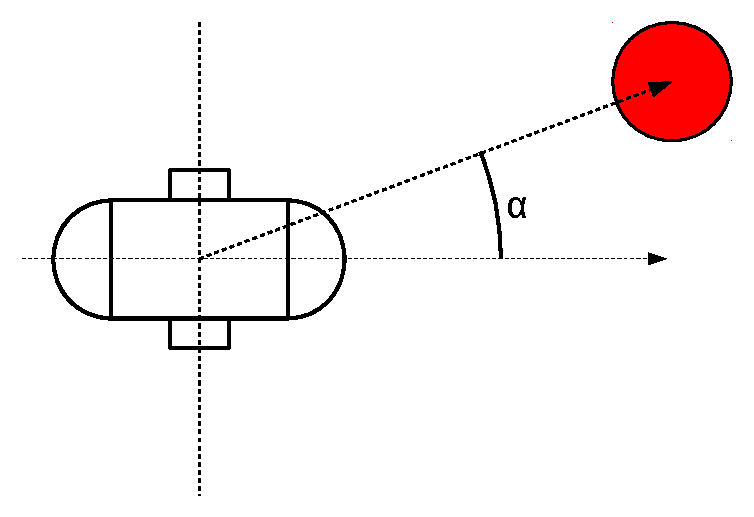
\includegraphics[width=\textwidth]{img/angle.pdf}
					\caption{Angle between robot head module and target.}
					\label{fig:angle}
				\end{figure}
				\onslide<3>
				\begin{figure}
					\centering
					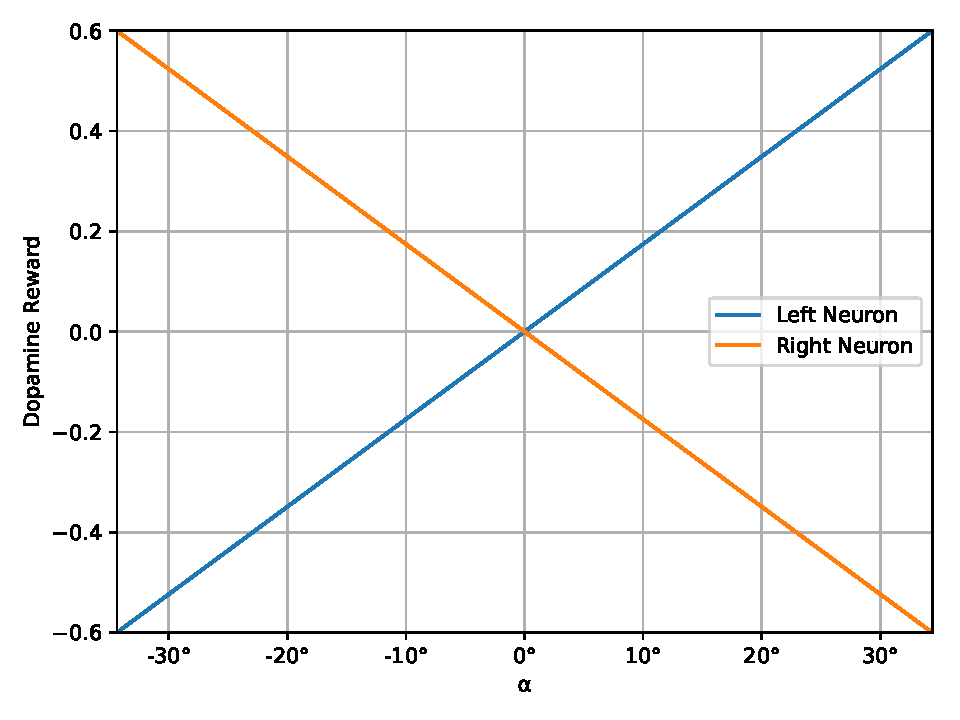
\includegraphics[width=\textwidth]{img/angle_reward.pdf}
					\caption{Target following reward function}
					\label{fig:angle_reward}
				\end{figure}
			\end{overprint}
	\end{columns}
\end{frame}

\begin{frame}
	\frametitle{Obstacle Avoidance SNN}
	\begin{columns}
		\column{0.5\linewidth}
			\begin{itemize}
				\item <1-> Four proximity sensors
				\item <2-> Proximity data preprocessing
				\item <3-> 4 Poisson input neurons
				\item <3-> Feed forward architecture
				\item <3-> Left and right LIF output neurons
			\end{itemize}
		\column{0.5\linewidth}
			\begin{overprint}
				\onslide<1>
				\begin{figure}
					\centering
					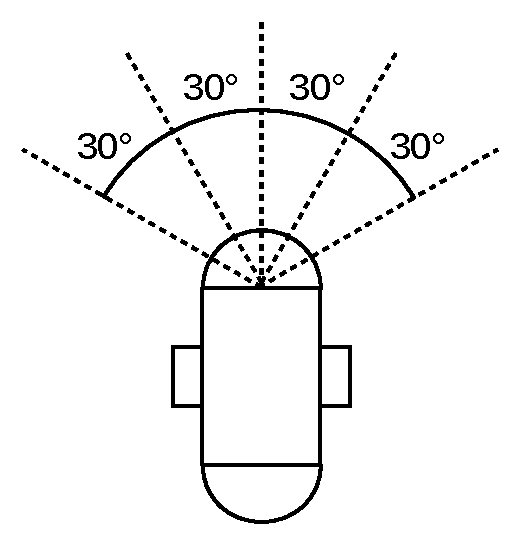
\includegraphics[height=0.7\textheight]{img/sensors_b.pdf}
					\caption{Proximity sensors}
					\label{fig:sensor_b}
				\end{figure}
				\onslide<2>
				\begin{itemize}
					\item Data in range $[0;3]$
					\item Mapped to range $[0:1]$
					\item $0$: No obstacle or at maximum distance
					\item $1$: Close obstacle
				\end{itemize}
				\onslide<3>
				\begin{figure}
					\centering
					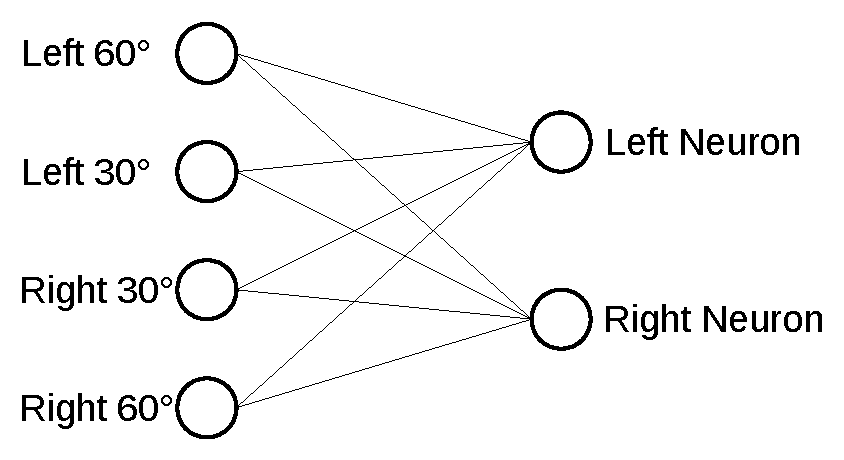
\includegraphics[width=\textwidth]{img/arch_oa.pdf}
					\caption{Obstacle avoidance SNN architecture}
					\label{fig:arch_oa}
				\end{figure}
			\end{overprint}
	\end{columns}
\end{frame}

\begin{frame}
	\frametitle{Obstacle Avoidance SNN cont.}
	\begin{columns}
		\column{\linewidth}
			\begin{itemize}
				\item <1-> Output interpreted as angle
				\[decode\left(n_{spikes}\right) = \frac{n_{spikes}}{n_{max}}\]
				\[\alpha = \alpha_{max} \left(n_l - n_r\right)\]
				\item <2-> Event based rewards on Episode failure
				\item <2-> Left and right neuron get the opposite rewards of each other
				\item <2-> 4 Reward cases, collision and target lost, obstacle left or right side
			\end{itemize}			
	\end{columns}
\end{frame}

\begin{frame}
	\frametitle{Controller Selection}
	\begin{itemize}
		\item Both SNN return an angle
		\item Select one as command for the robot
		\item Choose the target tracking angle except if that brings the robot too close to an obstacle.
	\end{itemize}
\end{frame}

\begin{frame}
	\frametitle{Training Environment}
	\begin{columns}
		\column{\linewidth}
			\begin{overprint}
				\onslide<1>
				\begin{figure}
					\centering
					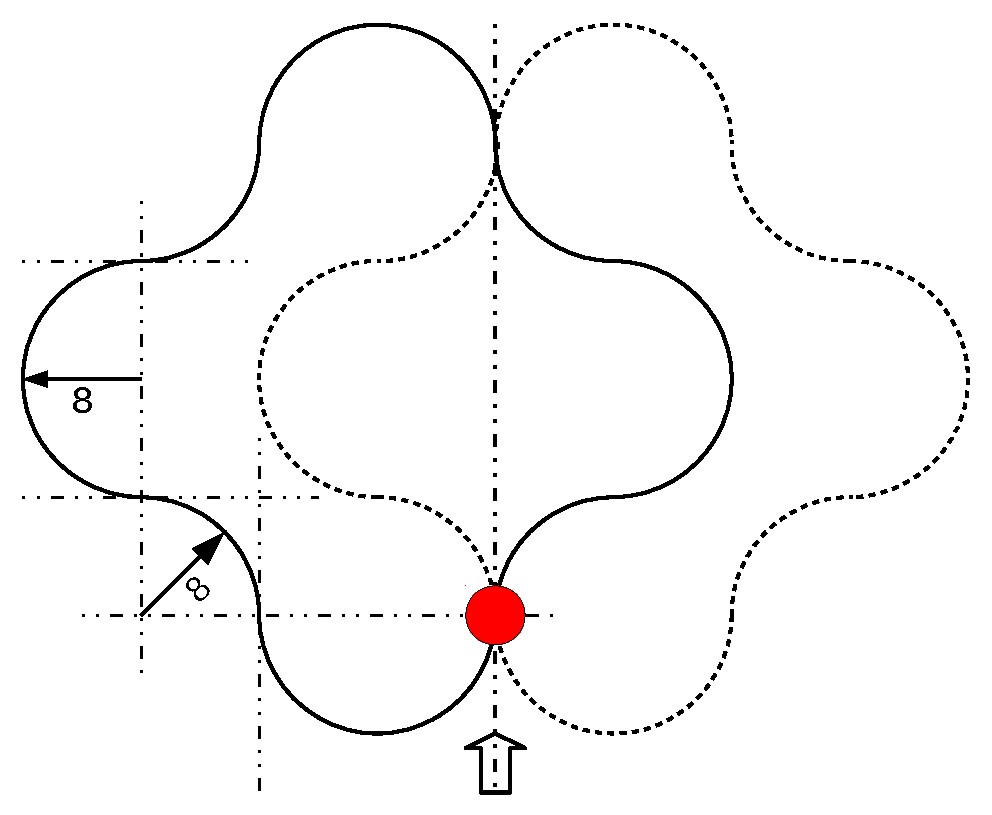
\includegraphics[height=0.6\textheight]{img/tf_training_path.pdf}
					\caption{Target tracking SNN training path}
					\label{fig:tf_training_path}
				\end{figure}
			\end{overprint}
	\end{columns}
\end{frame}

\begin{frame}
	\frametitle{Training Target Tracking SNN}
	\begin{figure}
		\centering
		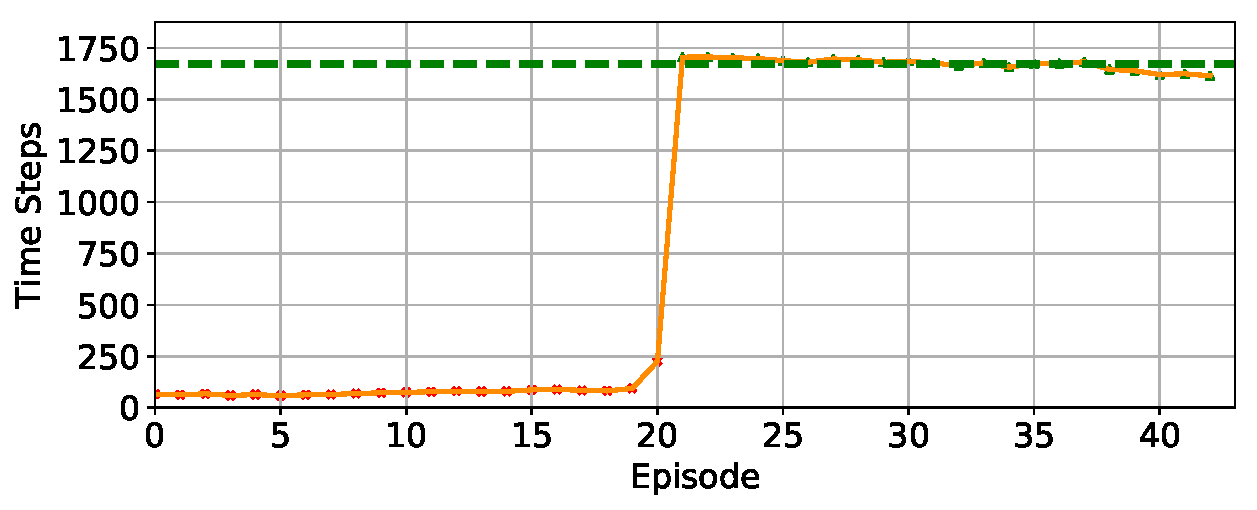
\includegraphics[width=\textwidth]{img/success_tf.pdf}
		\caption{Target Tracking Training}
		\label{fig:tf_success}
	\end{figure}
\end{frame}

\begin{frame}
	\frametitle{Training Target Tracking SNN}
	\begin{figure}
		\centering
		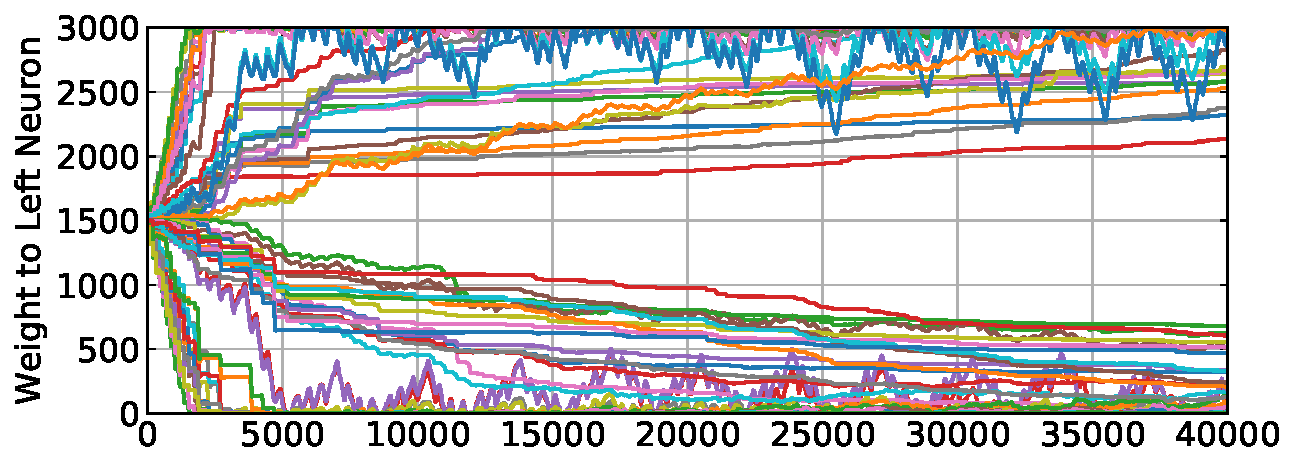
\includegraphics[width=\textwidth]{img/weight_change_left_tf.pdf}
		\caption{Left neuron weight changes during training}
		\label{fig:tf_weight_changes_left}
	\end{figure}
\end{frame}

\begin{frame}
	\frametitle{Training Environment}
	\begin{columns}
		\column{\linewidth}
			\begin{overprint}
				\begin{figure}
					\centering
					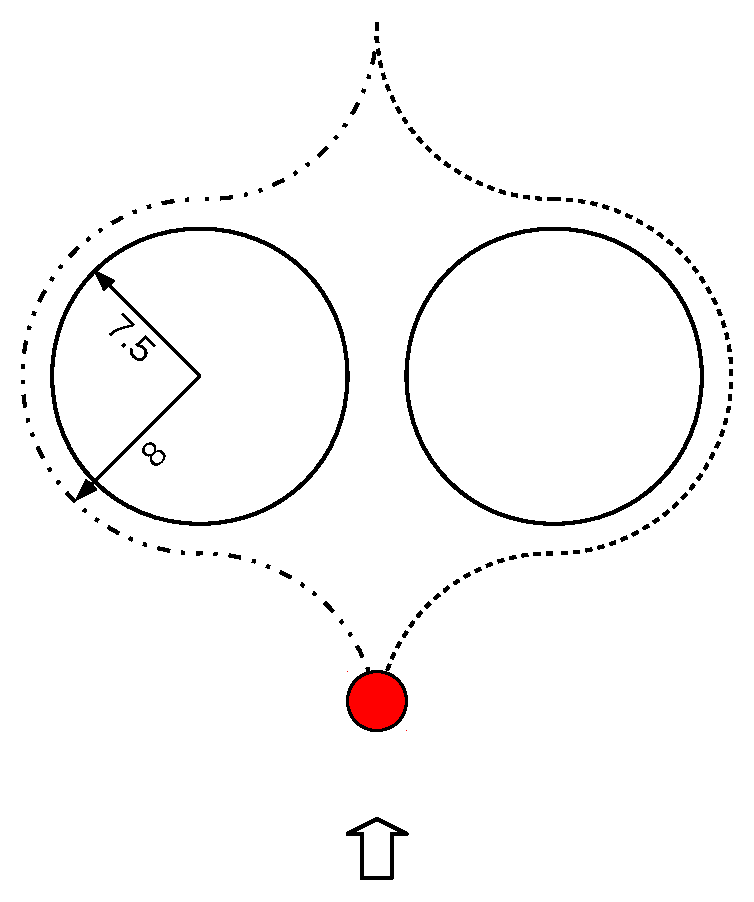
\includegraphics[height=0.6\textheight]{img/oa_training_path.pdf}
					\caption{Obstacle avoidance SNN training path}
					\label{fig:oa_training_path}
				\end{figure}
			\end{overprint}
	\end{columns}
\end{frame}

\begin{frame}
	\frametitle{Training Obstacle Avoidance SNN}
	\begin{figure}
		\centering
		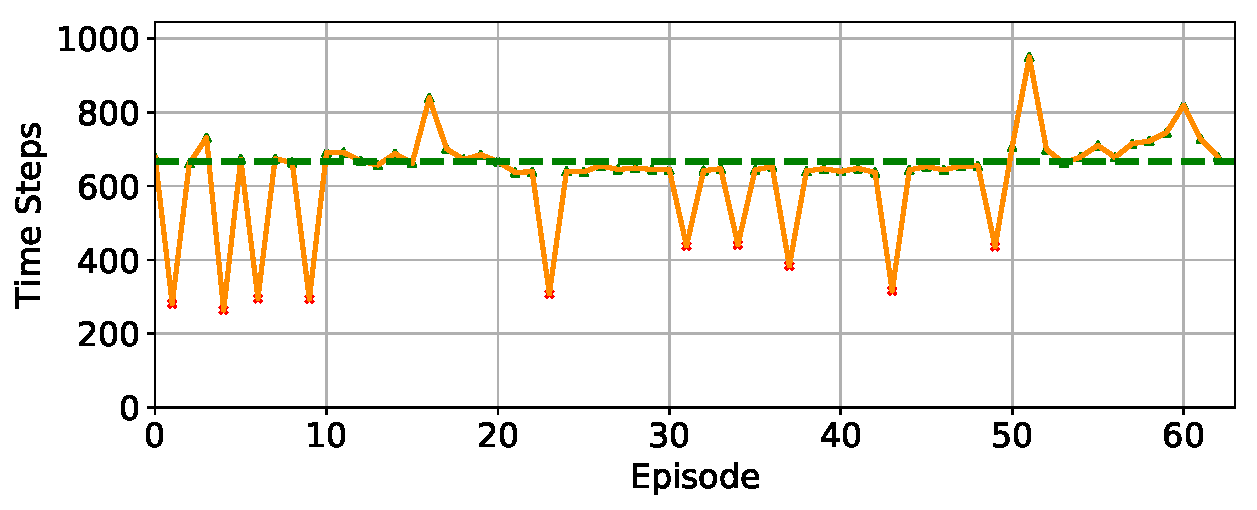
\includegraphics[width=\textwidth]{img/success_oa.pdf}
		\caption{Obstacle Avoidance Training}
		\label{fig:oa_success}
	\end{figure}
\end{frame}

\begin{frame}
	\frametitle{Training Target Tracking SNN}
	\begin{figure}
		\centering
		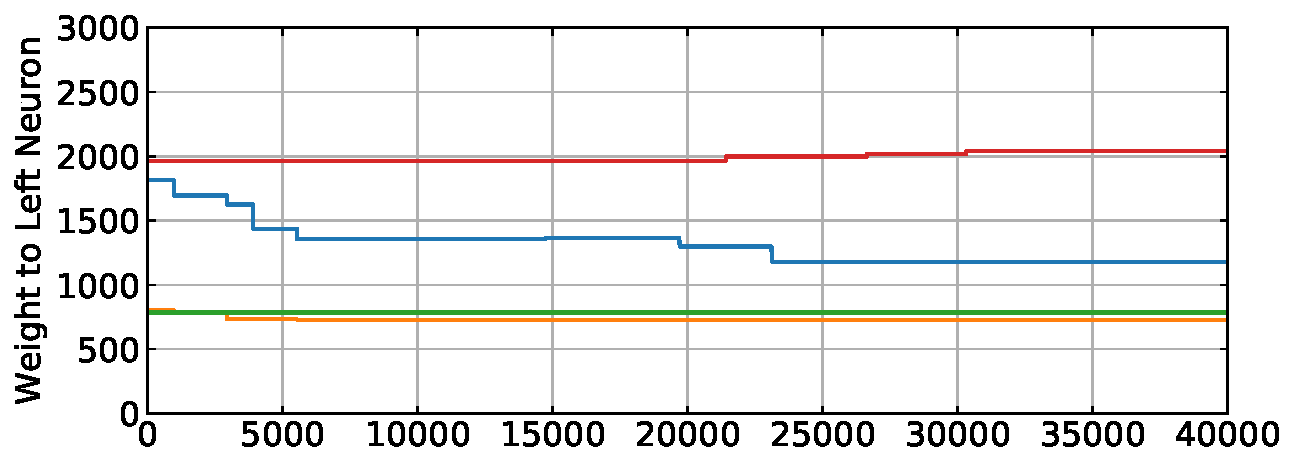
\includegraphics[width=\textwidth]{img/weight_change_left_oa.pdf}
		\caption{Left neuron weight changes during training}
		\label{fig:oa_weight_changes_left}
	\end{figure}
\end{frame}

\begin{frame}
	\frametitle{Evaluation}
	\begin{itemize}
		\item <1-> Average error $ e = \SI{7,39}{\degree}$
		\item <2-> Average error $ e = \SI{8.71}{\degree}$
	\end{itemize}
	\begin{overprint}
		\onslide<1>
		\begin{figure}
			\centering
			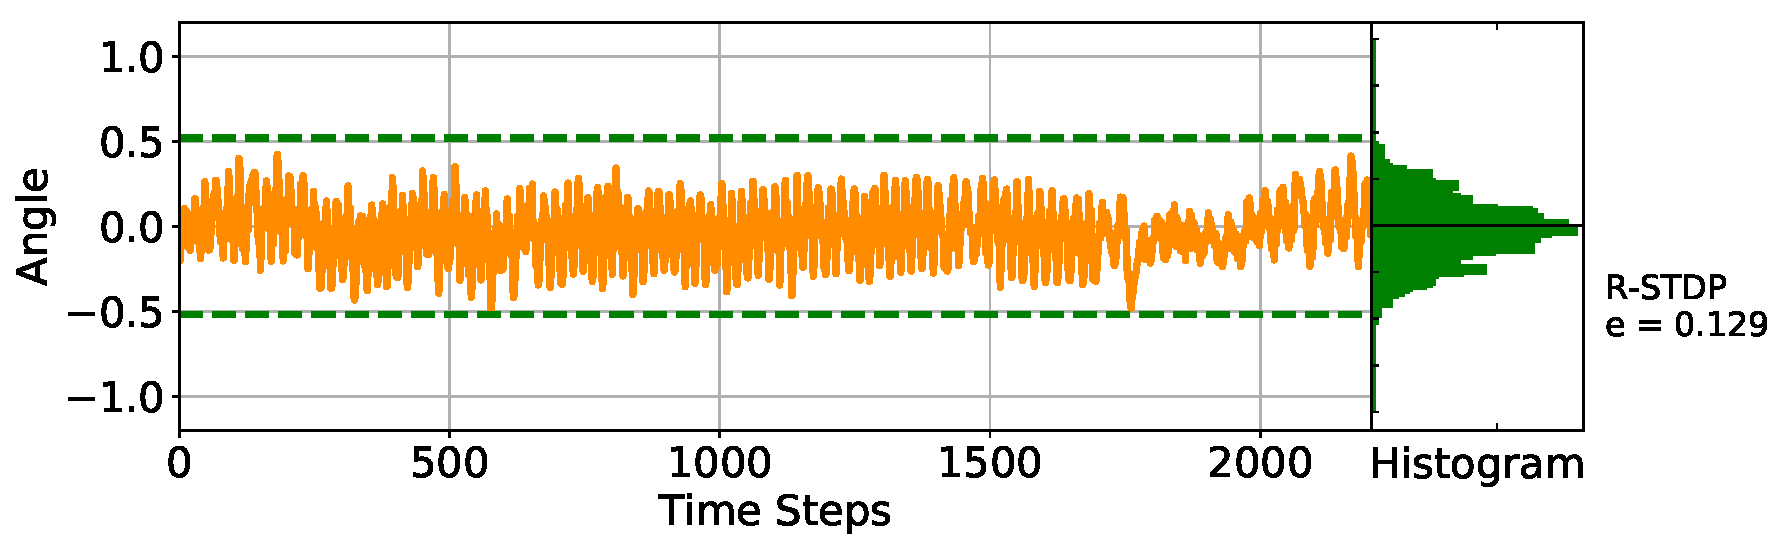
\includegraphics[width=\textwidth]{img/performance_tf.pdf}
			\caption{Performance on Target Following Task}
			\label{fig:Performance_tf}
		\end{figure}
		\onslide<2>
		\begin{figure}
			\centering
			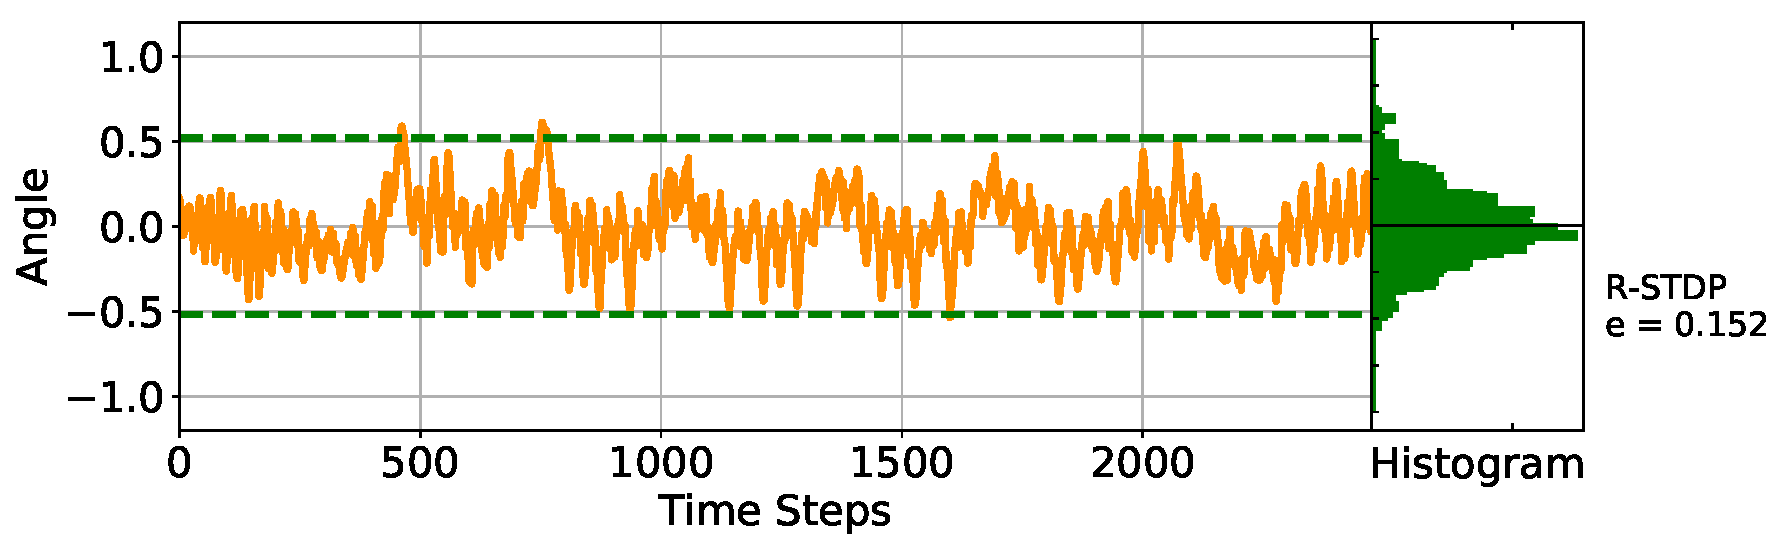
\includegraphics[width=\textwidth]{img/performance_oa.pdf}
			\caption{Performance on Target Tracking and Obstacle Avoidance Task}
			\label{fig:Performance_oa}
		\end{figure}
	\end{overprint}
\end{frame}

\begin{frame}
	\frametitle{title}
\end{frame}


% Include markdown source from ./pandoc
%
\begin{frame}
	\frametitle{Galileo - Weg zum Start}
	\begin{itemize}
		\item Antrag genehmigt am 14.4.1977
		\item Erforschung von Jupiter und seinen Monden
		\item Flugbahn\"anderungen durch Monde
		\item Raumsonde und Atmosph\"arenprobe
		\item Geplanter Start 1982
	\end{itemize}
\end{frame}


\begin{frame}
	\frametitle{Verteiltes Rechnen auf Galileo}
	\begin{itemize}
		\item CDS - Command and Data Subsystem
		\item DPU - Data Processing Units
		\item AACS - Attitude and Articulation Control Subsystem
		\item Atmosph\"arensonde System
		\item Systemsynchronisation über Clock alle 2.5 Millisekunden
	\end{itemize}
\end{frame}

\begin{frame}
	\frametitle{CDS - Command and Data Subsystem}
	\begin{itemize}
		\item CDS besteht aus HLM, zwei LLM und Bus
		\item HLM - High-level module
		\begin{itemize}
			\item RCA 1802, Speicher, Bussystem
			\item Bus kontrolle, System\"uberwachung
		\end{itemize}
		\item LLM - Low-level modules
		\begin{itemize}
			\item RCA 1802, Speicher
			\item \"Uberwachung der Raumsonde, Atmosph\"arenprobe
		\end{itemize}
		\item Identisches Backup
	\end{itemize}
\end{frame}

\begin{frame}
	\frametitle{CDS Software}
	\begin{itemize}
		\item Assembler mit Macros (IF, DO, ASSIGN)
		\item Vordergrund Prozesse z.B. Selbstest, Bus Kontrolle
		\item Hintergrundprozesse 6 Virtuelle Maschinen
		\item Jede VM hat einen Programmstack im Speicher
		\item VM mit höherer Priorität bekommen mehr Rechenzeit
	\end{itemize}
\end{frame}

\begin{frame}
	\frametitle{DPU - Data Processing Unit}
	\begin{itemize}
		\item Eine DPU pro Experiment
		\item RCA 1802 und Speicher
		\item Antenne im Time-Sharing Betrieb
		\item Anfallende Daten gehen im n\"achsten Zeitslot zur Erde
		\item Assembler
		\item Eine DPU wurde mit FORTH programmiert
	\end{itemize}
\end{frame}

\begin{frame}
	\frametitle{AACS - Attitude and Articulation Control Subsystem}
	\begin{itemize}
		\item Basiert auf Voyager's System
		\item Zwei redundande ATAC - Applied Technologies Advanced Computer
		\item Orientierung der Sonde im Raum
		\item Ausrichtung der Instrumentenplattform
		\item Z\"undung der Triebwerke
	\end{itemize}
\end{frame}

\begin{frame}
	\frametitle{AACS}
	\begin{itemize}
		\item 16 Bit Computer bestehend aus vier 4 Bit AMD 2900 bitslice Prozessoren
		\item 9,5 MHz
		\item HAL/S Programme
		\item Assembler Betriebssystem GRACOS - Galileo Real-time Attitude Control Operating System
		\item SEU Problem anf\"allig
		\item Ohne Versp\"atung beim Start Ausfall wegen Io m\"oglich
	\end{itemize}
\end{frame}

\begin{frame}
	\frametitle{RCA 1802}
	\begin{itemize}
		\item Strahlengeh\"artet Silizium auf Saphir
		\item 3.2 MHz Taktrate
		\item RISC mit 8 Bit Befehlen, nur 16 Befehle
		\item 16 Register zu je 16 Bit
		\item Programmcounter und Indexregister kann frei gew\"ahlt werden
		\item I/O direkt vom und in den Speicher
	\end{itemize}
\end{frame}


\begin{frame}
\frametitle{Start}
	\begin{itemize}
		\item Start verschoben in 1982, 1985 und 1986
		\begin{itemize}
			\item Verz\"ogerungen beim Spaceshuttle Programm
			\item Pr\"asident Reagan
			\item Challenger Katastrophe
		\end{itemize}
		\item Folgen jeder Verschiebung
		\begin{itemize}
			\item Neue Route zum Jupiter
			\item Umbau der Raumsonde
		\end{itemize}
		\item Start am 18.10.1989
	\end{itemize}
\end{frame}

\begin{frame}
\frametitle{Flug zum Jupiter \"Ubersicht}
	\begin{itemize}
		\item Dauer 6 Jahre
		\item Schwung holen an Venus und zwei mal an Erde
		\item Vorbeiflug an Planetoiden Gaspra und Ida
		\item Primärmission beginnt beim Jupiter
	\end{itemize}
\end{frame}


\begin{frame}
	\begin{figure}
		\centering
		\includegraphics[width=0.5\textwidth]{pics/venus.jpg}
		\caption{Vorbeiflug an Venus am 14.2.1990\cite{nasaphoto}}
		\label{VENUS}
	\end{figure}
\end{frame}

\begin{frame}
	\begin{figure}
		\centering
		\includegraphics[width=0.5\textwidth]{pics/erde0.jpg}
		\caption{Vorbeiflug an Erde am 12.12.1990\cite{nasaphoto}}
		\label{ERDE0}
	\end{figure}
\end{frame}

\begin{frame}
	\begin{figure}
		\centering
		\includegraphics[width=0.5\textwidth]{pics/gaspra.jpg}
		\caption{Vorbeiflug an Planetoiden Gaspra am 29.10.1991\cite{nasaphoto}}
		\label{GASPRA}
	\end{figure}
\end{frame}

\begin{frame}
	\begin{figure}
		\centering
		\includegraphics[width=0.7\textwidth]{pics/ida.jpg}
		\caption{Vorbeiflug an Planetoiden Ida und sein Mond Dactyl am 28.8.1991\cite{nasaphoto}}
		\label{IDA}
	\end{figure}
\end{frame}

\begin{frame}
	\begin{figure}
		\centering
		\includegraphics[width=0.7\textwidth]{pics/jupiter.jpg}
		\caption{Komet Shoemaker-Levy 9 schl\"agt auf Jupiter ein. 22.7.1994\cite{nasaphoto}}
		\label{JUPITER}
	\end{figure}
\end{frame}

\begin{frame}
	\begin{figure}
		\centering
		\includegraphics[width=0.8\textwidth]{pics/monde.jpg}
		\caption{Die Galileischen Monde Io, Europa, Ganymede, und Callisto\cite{nasaphoto}}
		\label{GALILEO_MONDE}
	\end{figure}
\end{frame}

\begin{frame}
	\frametitle{Probleme wärend der Reise zum Jupiter}
	\begin{itemize}
		\item HGA - Hochgewinnantenne Entfaltet sich nicht
		\item NGA - Niedriggewinnantenne nur \"Ubertragungsrate 10 Bit/s
		
		\item Bandrekorder reagiert für 18 Stunden nicht
		\item Leichter Schaden f\"uhrt zu 16\% weniger Speicher
	\end{itemize}
\end{frame}

\begin{frame}
	\frametitle{Probleml\"osung durch Software Updates}
	\begin{itemize}
		\item Antenne Paketbasierter Betrieb
		\item DPU's erstellen und w\"ahlen Pakete
		\item Bilder werden auf Bandrekorder zwischengespeichert
		\item CDS bearbeitet und komprimiert Bilder
		\item DCT - Diskrete Cosinustransformation zur verlustbehaftete Bildkomprimierung (JPEG)
	\end{itemize}
\end{frame}

\begin{frame}
\frametitle{Prim\"armission}
	\begin{itemize}
		\item 7.5.1995 bis 7.12.1997
		\item 11 Orbits um Jupiter
		\item Relativ naher Vorbeiflug an je einem Mond
		\item Unerwartet große Treibstoffreserven nach Mission
	\end{itemize}
\end{frame}

\begin{frame}
	\frametitle{Verl\"angerungen}
	\begin{itemize}
		\item GEM - Galileo Europa Mission
		\begin{itemize}
			\item 8.12.1997 bis 31.12.1999
			\item 14 Orbits, 7 Vorbeifl\"uge an Europa
		\end{itemize}
		\item GMM - Galileo Millennium Mission
		\begin{itemize}
			\item 1.2.2000 bis 21.9.2003
			\item Probleme h\"aufen sich
			\item Riskante Vorbeifl\"uge an Io
		\end{itemize}
	\end{itemize}
\end{frame}

\begin{frame}
	\frametitle{Vielen Dank f\"ur Ihre Aufmerksamkeit!}
	\begin{figure}
		\centering
		\includegraphics[width=0.6\textwidth]{pics/number_of_computers.png}
		\caption{xkcd Comic\cite{xkcd}}
		\label{NUMBER_OF_COMPUTERS}
	\end{figure}
\end{frame}


% Comment out if you do not want a bibliography
\begin{frame}[allowframebreaks]
    \bibliographystyle{abbrv}
    \setbeamertemplate{bibliography item}[text]
    \footnotesize
    \bibliography{lit}
\end{frame}

\end{document}



\begin{document}

% For lecture mode, you may want to build one set of slides per chapter but
% with common page numbering. If so,
% 1) create a new .tex file for each chapter, e.g. slides_chapN.tex,
% 2) set the part counter to N-1 (assuming chapters start at 0), and
% 3) and name your chapter by using the \part{} command.
%\setcounter{part}{-1}
%\part{Organisatorisches und Einleitung}

% Include source files from ./include (or ./include/chapN).

\begin{frame}
	\frametitle{Task: Target Tracking}
	\begin{columns}
		\column{0.5\linewidth}
			\begin{itemize}
				\item <1-> Target Tracking SNN
				\item <2-> Prevent collisions with walls
				\item <2-> Obstacle Avoidance SNN
				\item <2-> R-STDP learning rule
			\end{itemize}
		\column{0.5\linewidth}
			\begin{overprint}
				\onslide<1>
				\begin{figure}
					\centering
					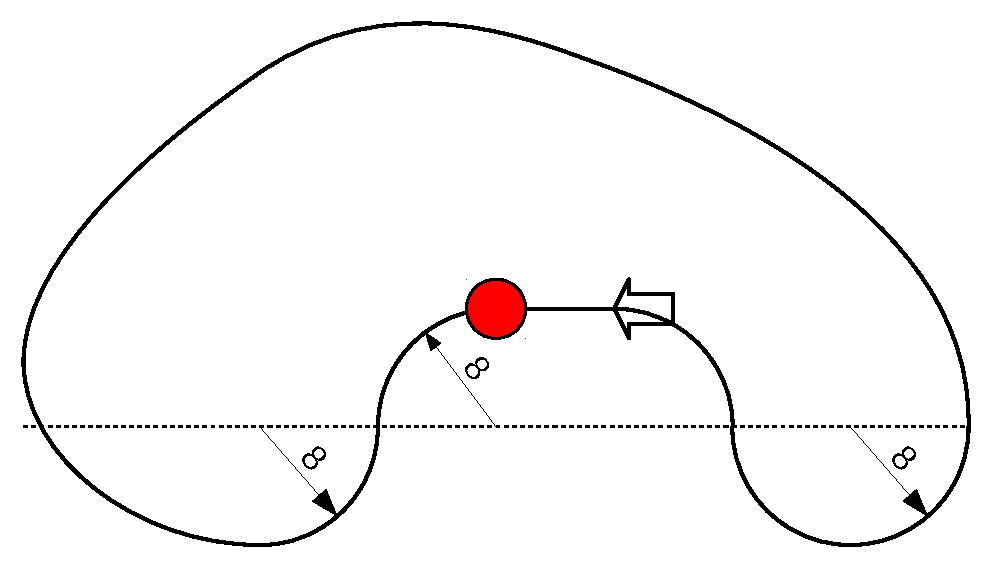
\includegraphics[width=\textwidth]{img/eval_path_tf.pdf}
					\caption{Target tracking SNN evaluation environment.}
					\label{fig:eval_path_tf}
				\end{figure}
				\onslide<2>
				\begin{figure}
					\centering
					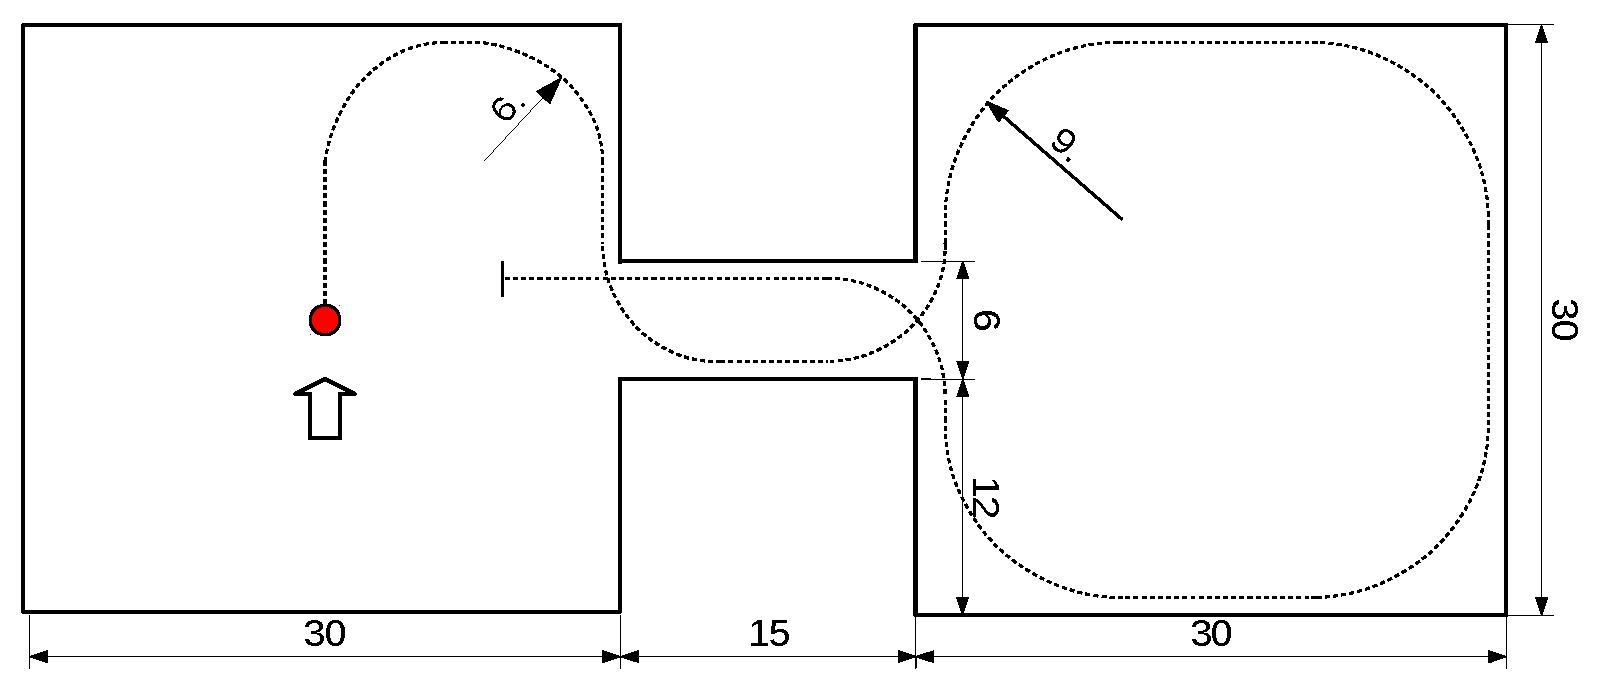
\includegraphics[width=\textwidth]{img/eval_path.pdf}
					\caption{Evaluation environment}
					\label{fig:eval_path}
				\end{figure}
			\end{overprint}
	\end{columns}
\end{frame}

\begin{frame}
	\frametitle{Target Following SNN}
	\begin{columns}
		\column{0.5\linewidth}
			\begin{itemize}
				\item <1-> Infrared image $32 \times 32 $ pixel resolution
				\item <2-> Image preprocessing
				\item <3-> 64 Poisson input neurons
				\item <3-> Feed forward architecture
				\item <3-> Left and Right LIF output neurons
			\end{itemize}
		\column{0.5\linewidth}
			\begin{overprint}
				\onslide<1>
				\begin{figure}
					\centering
					\includegraphics[height=0.7\textheight]{img/sensors_a.pdf}
					\caption{Infrared vision sensor}
					\label{fig:sensor_a}
				\end{figure}
				\onslide<2>
				\begin{figure}
					\centering
					\includegraphics[width=\textwidth]{img/img_pre.pdf}
					\caption{Image preprocessing in 3 steps}
					\label{fig:img_pre}
				\end{figure}
				\onslide<3>
				\begin{figure}
					\centering
					\includegraphics[width=\textwidth]{img/arch_tf.pdf}
					\caption{Target following SNN architecture}
					\label{fig:arch_tf}
				\end{figure}
			\end{overprint}
	\end{columns}
\end{frame}

\begin{frame}
	\frametitle{Target Following SNN cont.}
	\begin{columns}
		\column{0.5\linewidth}
			\begin{itemize}
				\item <1-> Output interpreted as angle
				\item <2-> Reward depends on Angle between head module and target
				\item <3-> Left and right neuron get the opposite rewards of each other
			\end{itemize}
		\column{0.5\linewidth}
			\begin{overprint}
				\onslide<1>
				\[decode\left(n_{spikes}\right) = \frac{n_{spikes}}{n_{max}}\]
				\[\alpha = \alpha_{max} \left(n_l - n_r\right)\]
				\[\alpha_t = c \alpha + \left(1 - c\right) \alpha_{t-1}\]
				\onslide<2>
				\begin{figure}
					\centering
					\includegraphics[width=\textwidth]{img/angle.pdf}
					\caption{Angle between robot head module and target.}
					\label{fig:angle}
				\end{figure}
				\onslide<3>
				\begin{figure}
					\centering
					\includegraphics[width=\textwidth]{img/angle_reward.pdf}
					\caption{Target following reward function}
					\label{fig:angle_reward}
				\end{figure}
			\end{overprint}
	\end{columns}
\end{frame}

\begin{frame}
	\frametitle{Obstacle Avoidance SNN}
	\begin{columns}
		\column{0.5\linewidth}
			\begin{itemize}
				\item <1-> Four proximity sensors
				\item <2-> Proximity data preprocessing
				\item <3-> 4 Poisson input neurons
				\item <3-> Feed forward architecture
				\item <3-> Left and right LIF output neurons
			\end{itemize}
		\column{0.5\linewidth}
			\begin{overprint}
				\onslide<1>
				\begin{figure}
					\centering
					\includegraphics[height=0.7\textheight]{img/sensors_b.pdf}
					\caption{Proximity sensors}
					\label{fig:sensor_b}
				\end{figure}
				\onslide<2>
				\begin{itemize}
					\item Data in range $[0;3]$
					\item Mapped to range $[0:1]$
					\item $0$: No obstacle or at maximum distance
					\item $1$: Close obstacle
				\end{itemize}
				\onslide<3>
				\begin{figure}
					\centering
					\includegraphics[width=\textwidth]{img/arch_oa.pdf}
					\caption{Obstacle avoidance SNN architecture}
					\label{fig:arch_oa}
				\end{figure}
			\end{overprint}
	\end{columns}
\end{frame}

\begin{frame}
	\frametitle{Obstacle Avoidance SNN cont.}
	\begin{columns}
		\column{\linewidth}
			\begin{itemize}
				\item <1-> Output interpreted as angle
				\[decode\left(n_{spikes}\right) = \frac{n_{spikes}}{n_{max}}\]
				\[\alpha = \alpha_{max} \left(n_l - n_r\right)\]
				\item <2-> Event based rewards on Episode failure
				\item <2-> Left and right neuron get the opposite rewards of each other
				\item <2-> 4 Reward cases, collision and target lost, obstacle left or right side
			\end{itemize}			
	\end{columns}
\end{frame}

\begin{frame}
	\frametitle{Controller Selection}
	\begin{itemize}
		\item Both SNN return an angle
		\item Select one as command for the robot
		\item Choose the target tracking angle except if that brings the robot too close to an obstacle.
	\end{itemize}
\end{frame}

\begin{frame}
	\frametitle{Training Environment}
	\begin{columns}
		\column{\linewidth}
			\begin{overprint}
				\onslide<1>
				\begin{figure}
					\centering
					\includegraphics[height=0.6\textheight]{img/tf_training_path.pdf}
					\caption{Target tracking SNN training path}
					\label{fig:tf_training_path}
				\end{figure}
			\end{overprint}
	\end{columns}
\end{frame}

\begin{frame}
	\frametitle{Training Target Tracking SNN}
	\begin{figure}
		\centering
		\includegraphics[width=\textwidth]{img/success_tf.pdf}
		\caption{Target Tracking Training}
		\label{fig:tf_success}
	\end{figure}
\end{frame}

\begin{frame}
	\frametitle{Training Target Tracking SNN}
	\begin{figure}
		\centering
		\includegraphics[width=\textwidth]{img/weight_change_left_tf.pdf}
		\caption{Left neuron weight changes during training}
		\label{fig:tf_weight_changes_left}
	\end{figure}
\end{frame}

\begin{frame}
	\frametitle{Training Environment}
	\begin{columns}
		\column{\linewidth}
			\begin{overprint}
				\begin{figure}
					\centering
					\includegraphics[height=0.6\textheight]{img/oa_training_path.pdf}
					\caption{Obstacle avoidance SNN training path}
					\label{fig:oa_training_path}
				\end{figure}
			\end{overprint}
	\end{columns}
\end{frame}

\begin{frame}
	\frametitle{Training Obstacle Avoidance SNN}
	\begin{figure}
		\centering
		\includegraphics[width=\textwidth]{img/success_oa.pdf}
		\caption{Obstacle Avoidance Training}
		\label{fig:oa_success}
	\end{figure}
\end{frame}

\begin{frame}
	\frametitle{Training Target Tracking SNN}
	\begin{figure}
		\centering
		\includegraphics[width=\textwidth]{img/weight_change_left_oa.pdf}
		\caption{Left neuron weight changes during training}
		\label{fig:oa_weight_changes_left}
	\end{figure}
\end{frame}

\begin{frame}
	\frametitle{Evaluation}
	\begin{itemize}
		\item <1-> Average error $ e = \SI{7,39}{\degree}$
		\item <2-> Average error $ e = \SI{8.71}{\degree}$
	\end{itemize}
	\begin{overprint}
		\onslide<1>
		\begin{figure}
			\centering
			\includegraphics[width=\textwidth]{img/performance_tf.pdf}
			\caption{Performance on Target Following Task}
			\label{fig:Performance_tf}
		\end{figure}
		\onslide<2>
		\begin{figure}
			\centering
			\includegraphics[width=\textwidth]{img/performance_oa.pdf}
			\caption{Performance on Target Tracking and Obstacle Avoidance Task}
			\label{fig:Performance_oa}
		\end{figure}
	\end{overprint}
\end{frame}

\begin{frame}
	\frametitle{title}
\end{frame}


% Include markdown source from ./pandoc
%
\begin{frame}
	\frametitle{Galileo - Weg zum Start}
	\begin{itemize}
		\item Antrag genehmigt am 14.4.1977
		\item Erforschung von Jupiter und seinen Monden
		\item Flugbahn\"anderungen durch Monde
		\item Raumsonde und Atmosph\"arenprobe
		\item Geplanter Start 1982
	\end{itemize}
\end{frame}


\begin{frame}
	\frametitle{Verteiltes Rechnen auf Galileo}
	\begin{itemize}
		\item CDS - Command and Data Subsystem
		\item DPU - Data Processing Units
		\item AACS - Attitude and Articulation Control Subsystem
		\item Atmosph\"arensonde System
		\item Systemsynchronisation über Clock alle 2.5 Millisekunden
	\end{itemize}
\end{frame}

\begin{frame}
	\frametitle{CDS - Command and Data Subsystem}
	\begin{itemize}
		\item CDS besteht aus HLM, zwei LLM und Bus
		\item HLM - High-level module
		\begin{itemize}
			\item RCA 1802, Speicher, Bussystem
			\item Bus kontrolle, System\"uberwachung
		\end{itemize}
		\item LLM - Low-level modules
		\begin{itemize}
			\item RCA 1802, Speicher
			\item \"Uberwachung der Raumsonde, Atmosph\"arenprobe
		\end{itemize}
		\item Identisches Backup
	\end{itemize}
\end{frame}

\begin{frame}
	\frametitle{CDS Software}
	\begin{itemize}
		\item Assembler mit Macros (IF, DO, ASSIGN)
		\item Vordergrund Prozesse z.B. Selbstest, Bus Kontrolle
		\item Hintergrundprozesse 6 Virtuelle Maschinen
		\item Jede VM hat einen Programmstack im Speicher
		\item VM mit höherer Priorität bekommen mehr Rechenzeit
	\end{itemize}
\end{frame}

\begin{frame}
	\frametitle{DPU - Data Processing Unit}
	\begin{itemize}
		\item Eine DPU pro Experiment
		\item RCA 1802 und Speicher
		\item Antenne im Time-Sharing Betrieb
		\item Anfallende Daten gehen im n\"achsten Zeitslot zur Erde
		\item Assembler
		\item Eine DPU wurde mit FORTH programmiert
	\end{itemize}
\end{frame}

\begin{frame}
	\frametitle{AACS - Attitude and Articulation Control Subsystem}
	\begin{itemize}
		\item Basiert auf Voyager's System
		\item Zwei redundande ATAC - Applied Technologies Advanced Computer
		\item Orientierung der Sonde im Raum
		\item Ausrichtung der Instrumentenplattform
		\item Z\"undung der Triebwerke
	\end{itemize}
\end{frame}

\begin{frame}
	\frametitle{AACS}
	\begin{itemize}
		\item 16 Bit Computer bestehend aus vier 4 Bit AMD 2900 bitslice Prozessoren
		\item 9,5 MHz
		\item HAL/S Programme
		\item Assembler Betriebssystem GRACOS - Galileo Real-time Attitude Control Operating System
		\item SEU Problem anf\"allig
		\item Ohne Versp\"atung beim Start Ausfall wegen Io m\"oglich
	\end{itemize}
\end{frame}

\begin{frame}
	\frametitle{RCA 1802}
	\begin{itemize}
		\item Strahlengeh\"artet Silizium auf Saphir
		\item 3.2 MHz Taktrate
		\item RISC mit 8 Bit Befehlen, nur 16 Befehle
		\item 16 Register zu je 16 Bit
		\item Programmcounter und Indexregister kann frei gew\"ahlt werden
		\item I/O direkt vom und in den Speicher
	\end{itemize}
\end{frame}


\begin{frame}
\frametitle{Start}
	\begin{itemize}
		\item Start verschoben in 1982, 1985 und 1986
		\begin{itemize}
			\item Verz\"ogerungen beim Spaceshuttle Programm
			\item Pr\"asident Reagan
			\item Challenger Katastrophe
		\end{itemize}
		\item Folgen jeder Verschiebung
		\begin{itemize}
			\item Neue Route zum Jupiter
			\item Umbau der Raumsonde
		\end{itemize}
		\item Start am 18.10.1989
	\end{itemize}
\end{frame}

\begin{frame}
\frametitle{Flug zum Jupiter \"Ubersicht}
	\begin{itemize}
		\item Dauer 6 Jahre
		\item Schwung holen an Venus und zwei mal an Erde
		\item Vorbeiflug an Planetoiden Gaspra und Ida
		\item Primärmission beginnt beim Jupiter
	\end{itemize}
\end{frame}


\begin{frame}
	\begin{figure}
		\centering
		\includegraphics[width=0.5\textwidth]{pics/venus.jpg}
		\caption{Vorbeiflug an Venus am 14.2.1990\cite{nasaphoto}}
		\label{VENUS}
	\end{figure}
\end{frame}

\begin{frame}
	\begin{figure}
		\centering
		\includegraphics[width=0.5\textwidth]{pics/erde0.jpg}
		\caption{Vorbeiflug an Erde am 12.12.1990\cite{nasaphoto}}
		\label{ERDE0}
	\end{figure}
\end{frame}

\begin{frame}
	\begin{figure}
		\centering
		\includegraphics[width=0.5\textwidth]{pics/gaspra.jpg}
		\caption{Vorbeiflug an Planetoiden Gaspra am 29.10.1991\cite{nasaphoto}}
		\label{GASPRA}
	\end{figure}
\end{frame}

\begin{frame}
	\begin{figure}
		\centering
		\includegraphics[width=0.7\textwidth]{pics/ida.jpg}
		\caption{Vorbeiflug an Planetoiden Ida und sein Mond Dactyl am 28.8.1991\cite{nasaphoto}}
		\label{IDA}
	\end{figure}
\end{frame}

\begin{frame}
	\begin{figure}
		\centering
		\includegraphics[width=0.7\textwidth]{pics/jupiter.jpg}
		\caption{Komet Shoemaker-Levy 9 schl\"agt auf Jupiter ein. 22.7.1994\cite{nasaphoto}}
		\label{JUPITER}
	\end{figure}
\end{frame}

\begin{frame}
	\begin{figure}
		\centering
		\includegraphics[width=0.8\textwidth]{pics/monde.jpg}
		\caption{Die Galileischen Monde Io, Europa, Ganymede, und Callisto\cite{nasaphoto}}
		\label{GALILEO_MONDE}
	\end{figure}
\end{frame}

\begin{frame}
	\frametitle{Probleme wärend der Reise zum Jupiter}
	\begin{itemize}
		\item HGA - Hochgewinnantenne Entfaltet sich nicht
		\item NGA - Niedriggewinnantenne nur \"Ubertragungsrate 10 Bit/s
		
		\item Bandrekorder reagiert für 18 Stunden nicht
		\item Leichter Schaden f\"uhrt zu 16\% weniger Speicher
	\end{itemize}
\end{frame}

\begin{frame}
	\frametitle{Probleml\"osung durch Software Updates}
	\begin{itemize}
		\item Antenne Paketbasierter Betrieb
		\item DPU's erstellen und w\"ahlen Pakete
		\item Bilder werden auf Bandrekorder zwischengespeichert
		\item CDS bearbeitet und komprimiert Bilder
		\item DCT - Diskrete Cosinustransformation zur verlustbehaftete Bildkomprimierung (JPEG)
	\end{itemize}
\end{frame}

\begin{frame}
\frametitle{Prim\"armission}
	\begin{itemize}
		\item 7.5.1995 bis 7.12.1997
		\item 11 Orbits um Jupiter
		\item Relativ naher Vorbeiflug an je einem Mond
		\item Unerwartet große Treibstoffreserven nach Mission
	\end{itemize}
\end{frame}

\begin{frame}
	\frametitle{Verl\"angerungen}
	\begin{itemize}
		\item GEM - Galileo Europa Mission
		\begin{itemize}
			\item 8.12.1997 bis 31.12.1999
			\item 14 Orbits, 7 Vorbeifl\"uge an Europa
		\end{itemize}
		\item GMM - Galileo Millennium Mission
		\begin{itemize}
			\item 1.2.2000 bis 21.9.2003
			\item Probleme h\"aufen sich
			\item Riskante Vorbeifl\"uge an Io
		\end{itemize}
	\end{itemize}
\end{frame}

\begin{frame}
	\frametitle{Vielen Dank f\"ur Ihre Aufmerksamkeit!}
	\begin{figure}
		\centering
		\includegraphics[width=0.6\textwidth]{pics/number_of_computers.png}
		\caption{xkcd Comic\cite{xkcd}}
		\label{NUMBER_OF_COMPUTERS}
	\end{figure}
\end{frame}


% Comment out if you do not want a bibliography
\begin{frame}[allowframebreaks]
    \bibliographystyle{abbrv}
    \setbeamertemplate{bibliography item}[text]
    \footnotesize
    \bibliography{lit}
\end{frame}

\end{document}

